% =============================================================================
\section{Introduction}
% * <stefano.panzeri@iit.it> 2016-06-16T20:30:54.633Z:
%
% > \section{Introduction}
%
% I did read this but i am not going to comment on it right now, i suggest to leave it for later
%
% ^.
% =============================================================================

SKETCH OF INTRODUCTION FROM SP

The cerebral cortex generates activity over a wide range of frequencies. Different frequencies are believed to have a different neural origin. In some cases different frequency ranges carry independent information about the stimuli. Different oscillations ranges seem to influence brain function, perception and regulate communication across neural populations. 

END OF SKETCH

The cortical column is widely regarded as the fundamental processing unit of the neocortex \citep{Mountcastle1957}.
Under this hypothesis, there is a common microcircuit spanning the depth of the cortex which is repeated across the cortical plane.
As the circuitry of the microcolumn is expected to have structural and functional similarities across the sensory modalities, therefore understanding this generic circuitry of the columnar computation will have far reaching impacts.
However, despite some progress towards understanding knowing the different types of neurons in present in different layers [CITATION], and the distribution of their most prominent inter-connections [CITATION], and a structural wiring diagram for the cortical microcircuit [CITATION], is still unknown.
Furthermore, the functional structure and computation of the microcircuit, which is to say the purpose of the processing in each cortical layer, is also still unknown.
In this paper, we aim to elucidate the functional structure of the cortical layers in \ac{V1} by examining the information contained in population activity at the various layers using \acp{LFP}.

\acp{LFP} are thought to reflect an integration of the membrane depolarisation in the neurons surrounding the electrode location.
The \ac{LFP} captures changes within the dendritic trees of neighbouring neurons as well as the soma.
The low frequency \ac{LFP} (XXXX \si{Hz}) captures slower changes in the population activity, and reflects more of the dendritic level of processing, integrated over a larger region than the high frequency \ac{LFP} \citep{Leski2013}.
%The idea of isolated frequency bands conveying complementary
Since early \ac{EEG} studies, it is has been hypothesized that different frequencies convey complementary information [CITATION] originates with \ac{EEG} studies, but and this has subsequently been extended to the \ac{LFP} [CITATION NEEDED].


We previously found that in the macaque \ac{V1} there are two \ac{LFP} frequency bands, \SIrange{1}{8}{Hz} and \SIrange{60}{100}{Hz}, which encode independent information in the macaque \ac{V1} about natural stimuli \citep{Belitski2008}.
In this study we expand the previous study by studying information as a function of cortical depth, and identify one aspect of natural scenes which is encoded differently by the two cortical frequency bands.
We hypothesised the two bands of information are generated through different cortical processes and originate at different locations in the cortex.
In this study we expand the previous study by studying information as a function of cortical depth, and identify one aspect of natural scenes which is encoded differently by the two cortical frequency bands.

Recent work has shown stimulation in \ac{V1} induces gamma activity in \ac{V4} (feedforward), whilst stimulation in \ac{V4} induces alpha oscillations in \ac{V1} (feedback) \citep{VanKerkoerle2014}.


% =============================================================================
\section{Experimental Methods}
% =============================================================================

\subsection{Ethics Statement}

Data was collected from \ac{V1} in four healthy rhesus monkeys (Macaca mulatta; four males \SIrange{8}{11}{kg}; \SIrange{10}{12}{years}).
All the experimental procedures were approved by the local authorities (Regierungspr\"asidium, Baden-W\"urttemberg, T\"ubingen, Germany; Project Number KY4/09) and were in full compliance with the guidelines of the European Community (EUVD 86/609/EEC) and were in concordance with the recommendation of the Weatherall report for the care and use of non-human primates \citep{Weatherall2006}.
The animals were group-housed in an enriched environment, under daily veterinarian care.
Weight, food and water intake were carefully monitored on a daily basis.


\subsection{Anesthesia for Neurophysiology Experiments}

The anesthesia protocol for all the experimental procedures have been described previously \citep{Logothetis1999,Logothetis2001}.
Briefly, glycopyrrolate (\SI{0.01}{mg.{kg}^{-1}}) and ketamine (\SI{15}{mg.{kg}^{-1}}), were used previous to general anesthesia.
Induction with fentanyl (\SI{3}{mg.{kg}^{-1}}), thiopental (\SI{5}{mg.{kg}^{-1}}) and succinylcholine chloride (\SI{3}{mg.{kg}^{-1}}), animals were intubated and ventilated using a Servo Ventilator 900C (Siemens, Germany) maintaining an end-tidal \ce{CO2} of \SIrange{33}{35}{mm.Hg} and oxygen saturation above \SI{95}{\percent}.

The anesthesia was maintained with remifentanil (\SIrange{0.5}{2}{\micro\gram.kg^{-1}.\min}) and mivacurium chloride (\SIrange{2}{6}{mg.kg^{-1}.h}) which ensured no eye movement during electrophygiological recordings.
The anesthetics dosage were established by measuring stress hormones and were selected to ensure unaffected physiological response at normal catecholamine concentrations \citep{Logothetis1999}.
In addition, it has been shown that using remifentanil has no significant effect on the neurovascular and neural activity of brain areas that do not belong to the pain matrix \citep{Goense2008,Zappe2008}.
In particular, visual cortex does not bind remifentanil.
We monitored the physiological state of the monkey continuously and kept within normal limits.
Body temperature was tightly maintained at \SIrange{38}{39}{\celsius}.
Throughout the experiment lactate Ringer's (Jonosteril, Fresenius Kabi, Germany) with \SI{2.5}{\percent} glucose was continuously infused at a rate of \SI{10}{ml.kg^{-1}.h^{-1}} in order to maintain an adequate acid-base balance and intravascular volume and blood pressure were maintained by the administration of hydroxyethyl starch as needed (Volulyte, Fresenius Kabi, Germany).

We used anesthetized animals because the preparation allows longer data acquisition times and to associate particular neural events to specific stimulus features without the strong effects of animal cognitive state, including effects of attention and arousal that would introduce additional complication in the interpretation of signals.


\subsection{Visual Stimulation}

A few drops of \SI{1}{\percent} cyclopentolate hydrochloride were used in each eye to achieve mydriasis.
Animals were wearing hard contact lenses (W\"ohlk-Contact-Linsen, Sch\"onkirchen, Germany) to focus the eyes on the stimulus plane.
The visual stimulation in all experimental sessions was presented in the eye with stronger ocular preference of recording sites.
The stimulus was presented using either an in-house custom-built projector (SVGA fibre-optic system with a resolution of \num{800x600} pixels, a frame rate of \SI{30}{Hz}), or a \ac{CRT} monitor (Iiyama MA203DT Vision Master Pro 513, frame rate \SI{118}{Hz}) placed at eye level, \SI{50}{\centi\metre} in front of the eye.
We found the same results with both display devices, except that monitor refresh with the \SI{30}{Hz} stimulus induced cortical oscillations at \SI{30}{Hz}.
Since this is the result of using an artificial stimulus with a low refresh rate (a well-known issue at this stimulus frequency), we removed this from the data (see Artefact Removal) and pooled the results across all sessions.
The visual stimulus consisted of high contrast (\SI{100}{\percent}), gamma corrected, fast-moving, colourful movie clips (no soundtrack) from commercially available movies.
Stimulus timings were controlled by a computer running a real-time OS (QNX, Ottawa, Canada).
Stimulus-on periods of \SI{120}{\second} (\num{5} sessions; \num{1} session: \SI{40}{\second}) were interleaved with stimulus-off periods (isoluminant grey screen) of \SI{30}{\second}.


\subsection{Neurophysiology Data Collection and Analysis}

The electrophysiological recordings were performed by doing a small skull trepanation, after which the dura was visualized with a microscope (Zeiss Opmi MDU/S5, Germany) and carefully dissected.
The electrodes were slowly advanced into the visual areas under visual and auditory guidance using manual micromanipulator (Narashige Group, Japan).
Electrodes consisted of laminar probes (NeuroNexus Technologies, Ann Arbor, USA).
These electrodes contained \num{16} contacts on a single shank \SI{3}{\milli\metre} long and \SI{150}{\micro\metre} thick.
The electrode sites were spaced at \SI{150}{\micro\metre} apart, with a recording area of \SI{413}{\micro\metre^2} each.
We used a flattened \ce{Ag} wire, which was positioned under the skin, as reference electrode \citep{Murayama2010}.
The recording access was filed with a mixture of \SI{0.6}{\percent} agar dissolved in \ce{NaCl} \SI{0.9}{\percent}, pH 7.4 solution which guaranteed good electrical connection between the ground contact and the animal \citep{Oeltermann2007760}.
The impedance of the contact points was always measured during the experiments and ranged from \SIrange{480}{800}{\kilo\ohm}.
The signals were amplified and filtered into a broadband of \SIrange{1}{8000}{Hz} (Alpha-Omega Engineering, Nazareth, Israel) and then digitized at \SI{20.833}{\kilo\Hz} with \SI{16}{bit} resolution (PCI-6052E; National Instruments, Austin, TX).


\acused{CRT}
\begin{table}[htbp]
\centering
\begin{tabular}{l l m{2.2cm} m{3.0cm} m{3.0cm}}
\toprule
Session &
    Display &
        Video frame rate (\si{fps}) &
            Artefact Frequencies Removed (\si{Hz}) &
                Size of \SI{1}{\degree} square in visual field\\
\midrule
\sesname{H05391} &
    Projector &
        \raggedleft \num{30.015} &
            \num{30} &
                \SI{16.0 x 16.0}{px}\\
\sesname{H05nm7} &
    Projector &
        \raggedleft \num{30.015} &
            \num{30}, \num{60} &
                \SI{21.3 x 21.3}{px}\\
\sesname{H05nm9} &
    \ac{CRT} &
        \raggedleft \num{118.098} &
            ~ &
                \SI{17.8 x 17.9}{px}\\
\sesname{E07nm1} &
    \ac{CRT} &
        \raggedleft \num{118.098} &
            \num{50}, \num{150} &
                \SI{17.9 x 17.8}{px}\\
\sesname{F10nm1} &
    Projector &
        \raggedleft \num{30.015} &
            \num{30}, \num{60} &
                \SI{21.3 x 21.3}{px}\\
\sesname{J10nm1} &
    \ac{CRT} &
        \raggedleft \num{118.098} &
            ~ &
                \SI{17.8 x 17.9}{px}\\
\bottomrule
\end{tabular}
\caption{%
\textit{Metadata for recording sessions.}
Stimuli were presented using either an in-house custom-built projector (SVGA fibre-optic system with a resolution of \num{800x600} pixels; ``Projector''), or a cathode ray tube monitor (Iiyama MA203DT Vision Master Pro 513; ``\ac{CRT}'') placed at eye level, \SI{50}{\centi\metre} in front of the eye.
Videos presented at \SI{118}{Hz} were up-sampled versions of the original \SI{30}{Hz} video, which was achieved by repeating each frame four times.
For artefact removal methodology, see \autoref{sec:lam_artefact}.
}
\label{tab:lam_md}
\end{table}


\subsection{Luminosity Function}

In order to best approximate the luminosity perceived by macaques, we relied on analogies with the human visual system.
Research in humans suggests the luminosity function is linearly related to the L- and M-cone activation, and independent of the S-cone activation \citep{Stockman2008}.
Furthermore, the weighting of L and M activations towards perceived luminance is believed to be similar to the L:M ratio in the individual \citep{Stockman2008}.
Old world monkeys such as macaques have an L:M ratio which is approximately 1:1 \citep{Dobkins2000}, so we assumed a luminosity function equally weighed between the L and M cone activations, $Y=L+M$.
The \SI{10}{\degree} cone fundamentals of \citet{Stockman2000} were used since the cone fundamentals of old world monkeys are known to be very similar to humans \citep{Dobkins2000}.
By taking the product of the emission spectra for pure red, green and blue with the luminosity function, integrating over wavelength and normalising, we obtained the following equations for relative luminance in terms of pixel intensity for the two devices used in the experiment.

\begin{align*}
    Y_{\text{projector}} &= 0.2171 \cdot R + 0.6531 \cdot G + 0.1298 \cdot B\\
    Y_{\text{CRT}}       &= 0.1487 \cdot R + 0.6822 \cdot G + 0.1691 \cdot B
\end{align*}


\subsection{Artefact Removal}
\label{sec:lam_artefact}

An artefact removal procedure was performed to reduce the effects of line noise (one session) and monitor refresh (the three sessions with \SI{30}{Hz} stimulus).
Artefact frequencies were identified by large, localised peaks in the power spectral density, which was computed with the periodogram method (see \autoref{tab:lam_md}).
In each case, the average artefact waveform was found and subtracted from the recorded signal.
To correct for phase shifts of the artefact, the averaging and subsequent subtraction were performed in blocks of 50 artefact periods with a phase chosen to maximise the cross-covariance of the signal with the artefact waveform.


\subsection{Current Source Density}

The \ac{CSD} was computed using the inverse \ac{CSD} method \citep{Pettersen2006}.
To compute this, we used a $\delta$-source model of local field generation with a diameter of \SI{500}{\micro\metre}, chosen to correspond to the effective size of columnar activity \citep{Horton2005,Lund2003}.
Since this method requires an even spacing between voltage measurements, gaps caused by faulty recording contacts in the electrode were filled in with a local average \citep{Wojcik2010}.
A homogeneous cortical conductivity of \SI{0.4}{\siemens\per\metre} was assumed \citep{Logothetis2007}.
The agar solution placed on top of the recording access point had an \ce{NaCl} concentration of \SI{9}{\mg\per\mL}, and the conductivity of this was estimated to be \SI{2.2}{\siemens\per\metre} \citep{Kandadai2012}.
The \ac{CSD} was spatially smoothed with a three-point Hamming filter.


\subsection{Multiunit Activity}

\autoref{fig:lam_1}: \ac{MUA} was calculated by band-passing the voltage recording between \SIrange{900}{3000}{Hz} with a zero-phase sixth-order Butterworth filter, taking the absolute value, applying a \SI{300}{Hz} low pass third-order Butterworth filter, and then downsampling.
This yields a smoothed spike rate, analogous to a population firing rate.

\autoref{fig:lam_3}: \ac{MUA} was calculated by downsampling by a factor of \num{3}, band-passing the voltage recording between \SIrange{900}{3000}{Hz} with a zero-phase sixth-order Butterworth filter, taking the absolute value, downsampling by a further factor of \num{12}.

\subsubsection{Multi-unit spiking activity}

Spikes were detected by high-pass filtering the raw signal above \SI{500}{Hz} with a zero-phase eighth-order Butterworth filter, and classifying any points more than 3.5 standard deviations above the mean signal during pre- and post-stimulus periods as a spike, with a minimum inter-spike-interval of \SI{1}{\milli\second}.

The majority of thalamic afferents in \ac{V1} stimulate \ac{L4} (albeit indirectly, see \citealp{Hansen2012}), with the first cortical response manifesting at layer 4C$\alpha$ \citep{Callaway1998}, resulting in an initial current sink and first burst of spiking activity located here.
Consequently, we confirmed the depth alignment of the electrodes by verifying that the initial current sink (\autoref{fig:lam_s1}C) and spiking activity (\autoref{fig:lam_s1}D) in response to stimulation both resided within the \ac{G} compartment.


\subsection{Receptive Field Locations}

The spatial \acp{RF} were found by reverse correlating the \ac{MUA} and the pixel-by-pixel Z-scored frame-by-frame difference in luminance with a fixed lag of \SI{66.7}{\milli\second}.
The rate of change in luminance was used because it is known to correlate well with thalamic drive.
For each session, the \ac{RF} centre was located using the average of the reverse correlation across all cortical channels.


\subsubsection{Nuclear magnetic resonance data collection}

For two of the four monkeys involved in the study, we made use of high-resolution \ac{NMR} anatomical scans (collected for a different experiment) to measure the cortical thickness at the recording site used (Supplemental \autoref{fig:lam_s1}A--B).

To estimate the cortical thickness at the recording site of the laminar electrodes, high-resolution \ac{NMR} anatomical scans were acquired at the vertical using a \SI{7}{T} scanner with a \SI{60}{\centi\metre} diameter bore (Bruker BioSpin GmbH, Ettlingen, Germany).
A custom-made chair was used to position the monkey in the magnet.
We used a single-shot gradient \ac{EPI} with a \ac{FOV} of \SI{96x96}{\milli\metre} and matrix of \num{256x256}.
We acquired 18 a thickness of \SI{1}{\milli\metre}, TE/TR 15/\SI{2000}{\milli\second} and flip angle of \SI{90}{\degree}.

Animal \sesname{H05} was found to have a cortical thickness of \SI{\sim 1.7}{mm} at the recording site, whilst \sesname{E07} had a thickness of \SI{\sim 1.56}{mm}.

The thickness of cortical material included in the \ac{SG}, \ac{G} and \ac{IG} components is \SI{\sim 0.3}{mm} more than the measured obtained from the \ac{NMR} recordings.
We believe this discrepancy is due to the inflammation of the cortex in response to the trauma of the electrode penetration and the non-perpendicularity of the electrode penetration angle.


\subsection{Identification of Cortical Laminae}

To identify the depth of each contact, we measured the potential evoked in response to the onset of the movie clip, and in response to full-screen maximum-luminance \SI{100}{\milli\second} flash stimuli with a \SI{6}{\second} interval.
From the measured potentials, we identified the boundary between the \ac{G} and \ac{IG} compartments as the source-sink reversal in the evoked \ac{CSD} (\citealp{Mitzdorf1979,Mitzdorf1985}; see Supplementary Materials).
We estimated the location of the boundary between the \ac{G} and \ac{SG} compartments by cross-referencing literature describing the average thickness of cortical laminae in Macaca mulatta, area 17 \citep{Lund1973,OKusky1982}.

\subsection{Aligning electrode penetrations}


\begin{figure}
\centering 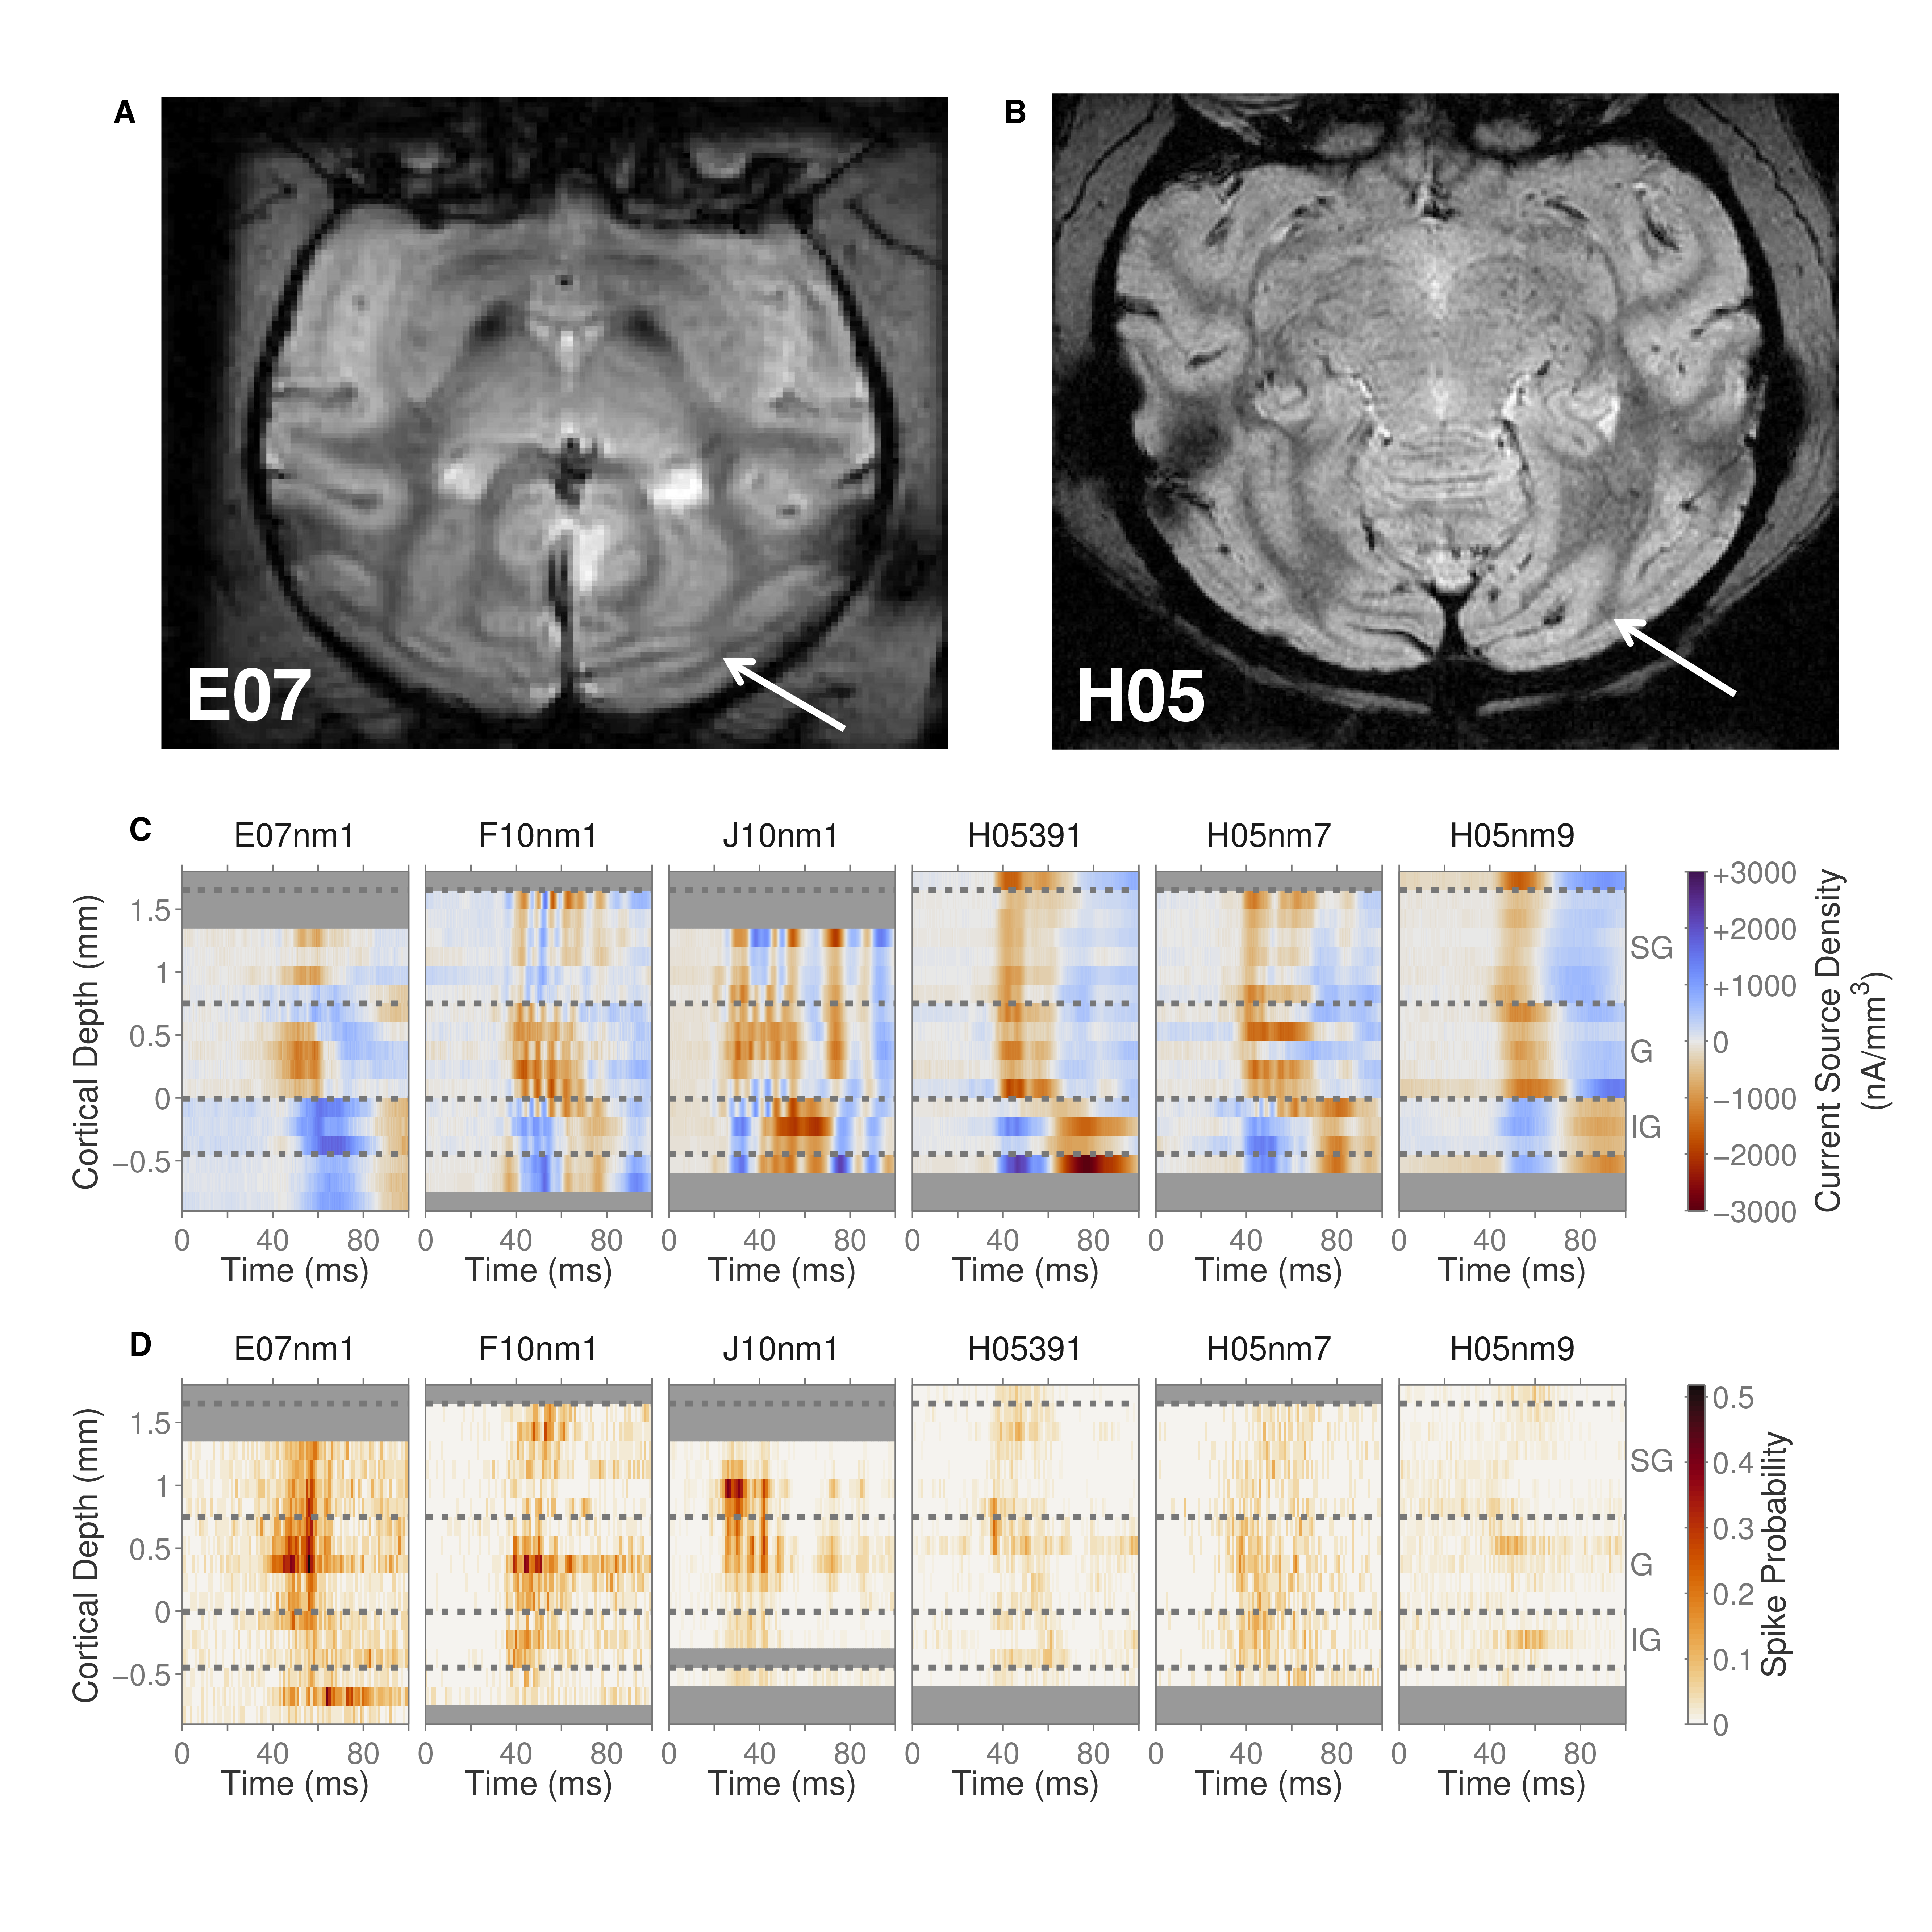
\includegraphics[width=\columnwidth]{paperfigs/figS1}
%
\caption{%
\textit{Electrode alignment.}
A--B: High resolution \ac{NMR} scans of two animals used to measure cortical thickness.
C: Stimulus triggered average \ac{CSD} responses, post-alignment.
For sessions \sesname{H05391}, \sesname{H05nm7}, \sesname{H05nm9} and \sesname{E07nm1}, the average response to onset of the movie stimulus is shown, whereas for sessions \sesname{F10nm1} and \sesname{J10nm1} the response to a full-field flash is shown.
D: Corresponding spike densities for the responses in panel C (\SI{1}{\milli\second} window duration).
}
\label{fig:lam_s1}
%
\end{figure}


For each recording session, the electrode was implanted in \iac{V1} at the recording site indicated in \autoref{fig:lam_s1}A--B.
The methodology for the insertion of the electrode is described in the Experimental Methods of the main text.

For each penetration, we endeavoured to align the electrode such that the most shallow electrode contact was at the boundary between cortical matter and the dura (near \ac{L1}).
However, this \textit{ad-hoc} method of alignment is unreliable, in part due to variation in cortical and laminar thickness both within between subjects.
Therefore, we performed \textit{post-hoc} realignment of the electrode contacts using the same methodology as \citet{Self2013,VanKerkoerle2014}.

To identify the depth of each contact, we measured the potential evoked in response to the onset of the movie clip, and in response to full-screen maximum-luminance \SI{100}{\milli\second} flash stimuli with a \SI{6}{\second} interval.
From the measured potentials, we identified the boundary between the \ac{G} and \ac{IG} compartments as the source-sink reversal in the evoked \ac{CSD} \citep{Mitzdorf1979,Mitzdorf1985}.
For this measurement, the \ac{CSD} was computed from the \ac{LFP} as described in Experimental Methods, but without spatially smoothing the signal with a Hamming filter.

The data from each electrode was re-aligned such that the source-sink reversal for each recording session was at a depth of \SI{0}{\milli\metre} (\autoref{fig:lam_s1}C).
We estimated the location of the boundary between the \ac{G} and \ac{SG} compartments by cross-referencing literature describing the average thickness of cortical laminae in Macaca mulatta, area 17 \citep{Lund1973,OKusky1982}.

The validity of this choice of alignment of electrode penetrations was then tested by considering the average response in spiking activity to the onset of the stimulus, and by measuring the cortical thickness at the recording site using \ac{NMR}.


\subsection{Power as a function of depth and frequency}

To compute power and information as a function of temporal frequency, the cortical data (\ac{LFP} and \ac{CSD}) were filtered in a series of bands each with a fractional bandwidth of \SI{50}{\percent}, because cortical power falls off rapidly with frequency in a \nicefrac{1}{f} relationship.
Each successive band begins and ends with frequencies 1.291 times higher than the last, so that each band has \SI{0}{\percent} overlap with bands further away than its immediate neighbours and a \SI{44}{\percent} and \SI{56}{\percent} overlap with its preceding and succeeding bands respectively.
The data was filtered with a zero-phase sixth-order Butterworth filter, after which the instantaneous power was estimated by taking the squared absolute value of the Hilbert transform.
The power in each band was integrated over a series of \SI{50}{\milli\second} windows, centred at the time of each frame change in the movie (once every \SI{33}{\milli\second}, leading to a \SI{50}{\percent} overlap of neighbouring windows).
The power in the \SIrange{4}{16}{Hz} and \SIrange{60}{170}{Hz} bands was computed similarly.
\autoref{fig:lam_3}A--B are plotted with power values averaged over all windows and trials, then expressed in decibels relative to the average power \SIrange{1.5}{248}{Hz} (estimated by summing the power in alternate bands).
Throughout \autoref{fig:lam_3} and \autoref{fig:lam_s3}, datapoints are shown at the band centres.


\subsection{Information as a function of depth and frequency}

Power in each band was computed as above, then for each frequency band and depth we took a \num{10}-bin histogram of the power across all the \SI{50}{\milli\second} windows for all repetitions.
The bin edges were chosen such that \SI{10}{\percent} of the distribution fell into each bin, and the identity of which bin the window was allocated into was taken to be its ``stimulus''.
We found the mutual information between the response and which frame was on screen at that time --- the ``stimulus'' --- by computing the Shannon information using the information breakdown toolbox \citep{Magri2009}.
Bias due to undersampling was corrected for using the \ac{PT} method \citep{Treves1995}.
Each information calculation was also bootstrapped \num{20} times with a randomly shuffled mapping of stimulus to response (also bias-corrected).
To ensure the amount of information was statistically significant, we checked each information estimate exceeded the bootstrap mean by more than \num{3} standard deviations of the bootstrap values.
The bootstrap mean was then subtracted from the estimated information, to counter any residual bias.


\subsection{Cortical Distribution of Power}

For each session, the distribution of power across the cortical depth (Figures \ref{fig:lam_power_lfp} and \ref{fig:lam_power_csd}, right-hand insets) was determined by normalising the power at each depth by the summed power across all cortical depths for that band.
We then took an average across sessions, weighted by the number of cortical recording sites in each session to prevent faulty (omitted) electrode contact sites from distorting the result.


\subsection{Information Redundancy}

Information redundancy was computed with the same stimuli windows as used in the information calculations.
However, for this calculation power was binned using only \num{3} bins, each containing a third of the power datapoints across all repetitions of the movie stimulus.
Let $S$ denote the set of stimuli, and let $X$ and $Y$ each be the set of powers during each stimulus in one of the frequency bands at a particular depth.
The information in each $\I\left(X;S\right)$ and $\I(Y;S)$ was computed in the same manner as above.
The information in the joint distribution $\I(\left\{X,Y\right\};S)$ was computed by considering each combination of the binned $X$ and $Y$ as a different response, yielding a total of \num{9} different responses for $\{X,Y\}$.

The relative redundancy is then defined as
\begin{equation*}
\operatorname{Redundancy}=\frac{\I\left(X;S\right)+\I\left(Y;S\right)-\I\left(\left\{X,Y\right\};S\right)}{\I\left(\left\{X,Y\right\};S\right)}
\end{equation*}
and was computed using the information breakdown toolbox \citep{Magri2009}.


\subsection{Noise and signal correlations}

Noise and signal correlation were both computed by binning the cortical response into bins of duration \SI{50}{\milli\second} following every frame change in the movie.
For the signal correlation, responses were averaged over repetitions to give a single mean response to each frame.
The set of cortical responses in a given frequency band and depth was correlated against the responses at another frequency band and depth using the Pearson correlation coefficient.

Noise correlation was computed by taking the set of responses in two different bands to a single frame onset and correlating their responses.
This was repeated for each frame, and the average over all frames was computed.
In each case, the analysis process was repeated with a shuffled pairing of responses in order to perform bootstrap statistics.
Correlation coefficients which were less than three standard deviations of the bootstraps from the bootstrap mean are shown as white in \autoref{fig:lam_s3}.


\subsection{Information about Spatial Components}

The method to find the change in luminance in each spatial frequency band is illustrated in \autoref{fig:lam_4}.
First, we took the two-dimensional fast-Fourier transform of a \SI{224}{px} square from the movie.
A fourth-order Butterworth filter with a width of one octave was applied using a mask in the Fourier domain, and the result was projected back to the spatial domain.
We then took the pixel-wise difference between each spatially filtered pair of consecutive frames.
To provide a measure of the amount of change in luminance at this spatial resolution, we took the absolute amount of change in each pixel and summed this within a \SI{2}{\degree} diameter circular window centred at the receptive field location.

Applying this to the entire movie provided a temporal sequence of luminance changes in each spatial range.
Similar to before, we took a \num{10}-bin histogram and took the identity the bin in which each luminance change fell to be the ``stimulus''.
The mutual information between this stimulus and the neural response --- the power within \SIrange{4}{16}{Hz} and \SIrange{60}{170}{Hz} frequency bands --- was computed with a \SI{67}{\milli\second} lag between stimulus and response.


\subsection{Information about Fine and Coarse Luminance Changes}

Coarse and fine luminance changes in the stimulus were isolated in the same manner as the spatial components above, but using a low-pass (\SI{<0.3}{\cpd}) and high-pass (\SI{>1}{\cpd}) fourth-order Butterworth filter respectively.
For both the \SIrange{4}{16}{Hz} and \SIrange{60}{170}{Hz} \ac{CSD} powers, we computed the correlation and mutual information with the coarse and fine luminance changes, and averaged across sessions.


\subsection{Information lag between granular and infragranular compartments}

The information about fine and coarse stimuli contained in \SIrange{4}{16}{Hz} and \SIrange{60}{170}{Hz} neural frequency bands was computed as a function of the lag between stimulus and response, in steps of \SI{1.73}{\milli\second}.
For each cortical recording depth, we found determined the latency of the response as the lag which gave the maximum amount of information about the stimulus.
This step was performed for each session individually.
Since differences in latency from stimulation to \ac{V1} were larger between different sessions than between different depths for the same session, we found for each session and each frequency band the overall latency as the mean latency across all cortical depths.
For each session, we then subtracted its overall latency from the distribution of latencies across the cortical depth to create zero-centred distributions across recording depths.
From the zero-centred latency distributions we then computed the average relative latency and its standard error across sessions.
To make the data easier to conceptualise, for \autoref{fig:lam_6}C the average overall latency across sessions was added back to each trace.

To perform the statistical test, the relative latency was averaged across the five electrode contacts in \ac{IG} and also averaged across the three contacts in \ac{G}.
A paired $t$-test was performed across all \num{6} sessions to test whether the maximum information in the \ac{G} compartment consistently occurred earlier than information in the \ac{IG} compartment.

For \autoref{fig:lam_6}D, the difference in information latency between each pairs of electrode depths was tested for statistical significance using a paired $t$-test, with insignificant differences shown in white.


\subsection{Cross-Frequency Phase-Amplitude Coupling}

Strength of cross-frequency coupling was measured using the Modulation Index \citep{Tort2010}.
\ac{CSD} data was filtered for two bands, \SIrange{4}{16}{Hz} and \SIrange{60}{170}{Hz}, using a zero-phase sixth-order Butterworth filter, and the instantaneous phase of \SIrange{4}{16}{Hz} and envelope amplitude of \SIrange{60}{170}{Hz} were each estimated using a Hilbert transform.
We took a histogram of the \SIrange{4}{16}{Hz} phase datapoints with \num{16} bins each of width $\nicefrac{\pi}{8}$ radians, and took the average of the \SIrange{60}{170}{Hz} amplitudes simultaneous with the phase datapoints in each bin.
This provides a distribution of amplitude at one depth as a function of phase at another.
The Modulation Index is then the normalised Kullback-Leibler divergence of this distribution from a uniform distribution.


% =============================================================================
\section{Results}
% =============================================================================

To understand how oscillatory activity at different layers of \acf{V1} encodes naturalistic visual information, we recorded neural activity in cortical area \acs{V1} with a multi-contact laminar electrode array in four monkeys (Macaca mulatta), anaesthetized with opiates.
The animals were presented with a clip from a Hollywood movie which lasted \SI{30}{\second} or \SI{120}{\second} and was repeated \numrange{40}{150} times, depending on session (see Experimental Methods).

Each electrode housed \num{16} equally spaced (\SI{150}{\micro\metre}) contacts spanning a total depth of \SI{2250}{\micro\metre}, and was inserted perpendicular to the cortical surface (\autoref{fig:lam_1}A).
We recorded broadband \acp{LFP} from each electrode contact, and used the \acp{LFP} to compute at each electrode location the \ac{CSD}, a measure of the local flow of charge at any given point \citep{Einevoll2013}.
To align the depth of the electrodes across recording sessions, we identified the border between Layer 4 and 5 as the inversion of the \ac{CSD} from sink to source in response to the onset of visual stimulation (see \citealp{Schroeder1991}, and \autoref{fig:lam_s1}).
We then divided the cortical depth into \acf{G}, \acf{SG}, and \acf{IG} compartments (see Experimental Methods for details).

In order to identify the spatial area of the movie stimulus that modulated the neural activity that we recorded, we estimated the spatial \ac{RF} of the \ac{MUA} recorded in each electrode contact site by reverse-correlating the rate of change of luminance of each pixel in the movie with the \ac{MUA}.
The spatial-\ac{RF} locations that we identified (see \autoref{fig:lam_1}B for an example session) did not vary with depth, confirming the perpendicularity of the electrode penetration and that all electrode contacts were recording from the same cortical column.


\begin{figure}[htbp]
\centering 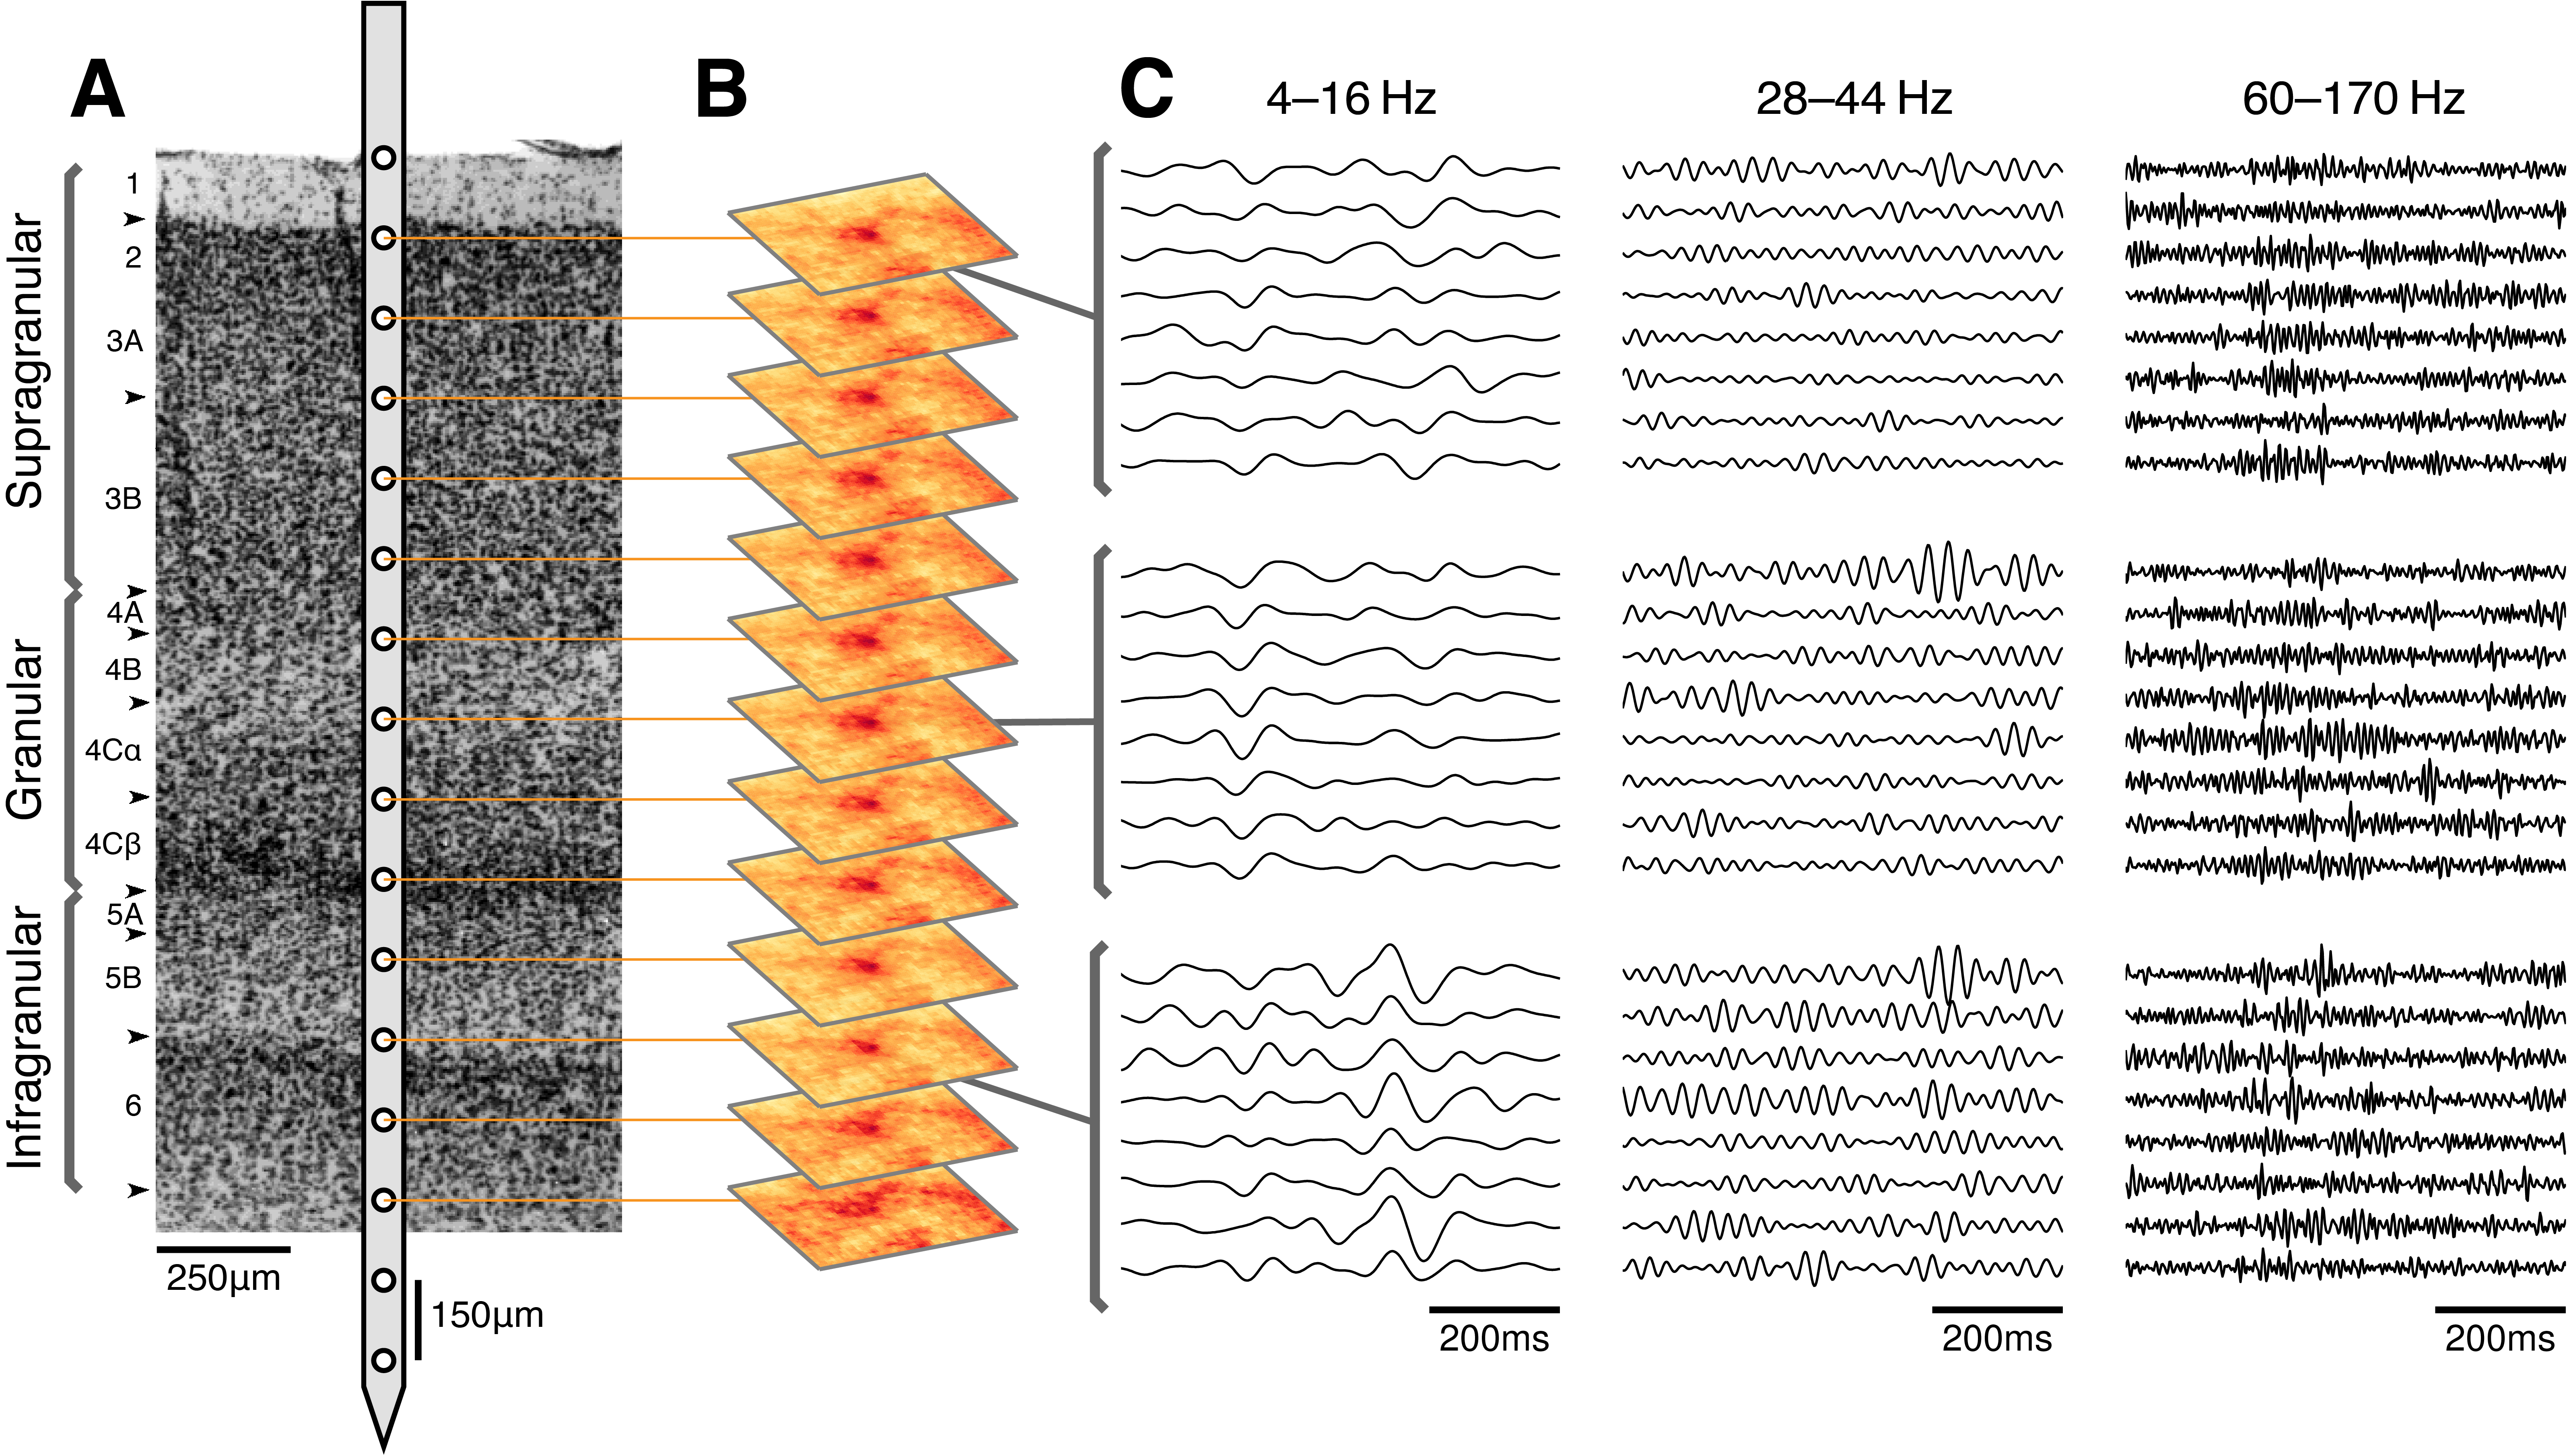
\includegraphics[width=\columnwidth]{paperfigs/fig1}
%
\caption{%
\textit{Overview of data collection and example data.}
A: Illustration of experimental recording setup, showing approximate locations of electrode contacts in relation to a Nissl stained section of macaque \ac{V1} cortex.
Boundaries between cortical laminae are indicated with arrowheads.
(Stain reproduced from \cite{Tyler1998}.)
(Note: Electrode width is not to scale.)
B: Receptive field locations were consistent across the cortical depth.
Location of receptive field for each cortical recording site was identified by reverse correlating the \ac{MUA} with the luminance changes of each pixel in the movie (session \sesname{E07nm1}).
C: Example \ac{CSD} traces from simultaneous recordings at three cortical depths for eight repetitions of a movie fragment (session \sesname{H05nm7}).
The data are split into three temporal frequency bands (\SIrange{4}{16}{Hz}, \SIrange{28}{44}{Hz} and \SIrange{60}{170}{Hz}, see Methods).
}%
\label{fig:lam_1}
%
\end{figure}


\subsection{Distribution of information across depth and frequency}

We considered how neural activity in different frequency bands changed in response to the movie.
To visually convey how information is encoded into different frequency bands (\autoref{fig:lam_1}C), we filtered the \ac{CSD} at three cortical depths in three spectral bands (\SIrange{4}{16}{Hz}, \SIrange{28}{44}{Hz} and \SIrange{60}{170}{Hz}), during eight presentations of a portion of the movie clip.

Within this small sample of the overall dataset, one can observe that large, low-frequency deflections in the activity are consistent across trials within \ac{G} and \ac{IG} depths, and the envelope-amplitude of activity in the \SIrange{60}{170}{Hz} band is also consistent across trials, most clearly for the \ac{SG} compartment.
Activity in the \SIrange{28}{44}{Hz} range was more variable across trials for any cortical depth, and did not seem to be stimulus modulated.


\begin{figure}[htbp]%
    \centering
    \hspace*{\fill}
    \subfloat[][\acs{LFP} power.\label{fig:lam_power_lfp}]{%
        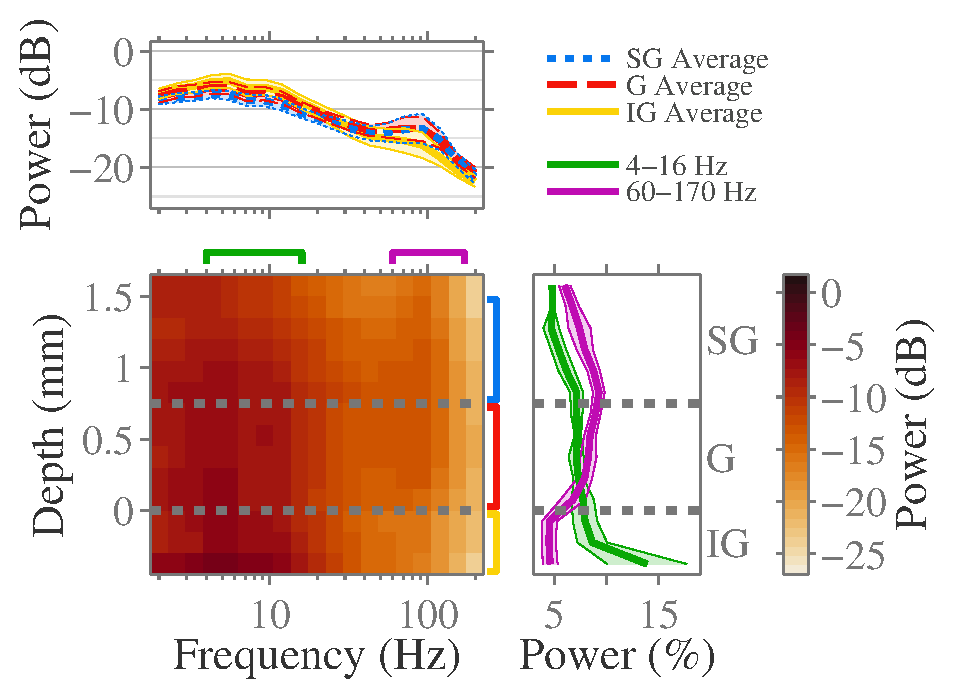
\includegraphics[scale=.45]{%
figs/info/fig3set-logRsp-Cln-power-straightnangeomean-compzonescb-legend.eps}}
    \hspace*{\fill}\hspace{.2cm}\hspace*{\fill}
    \subfloat[][\acs{CSD} power.\label{fig:lam_power_csd}]{%
        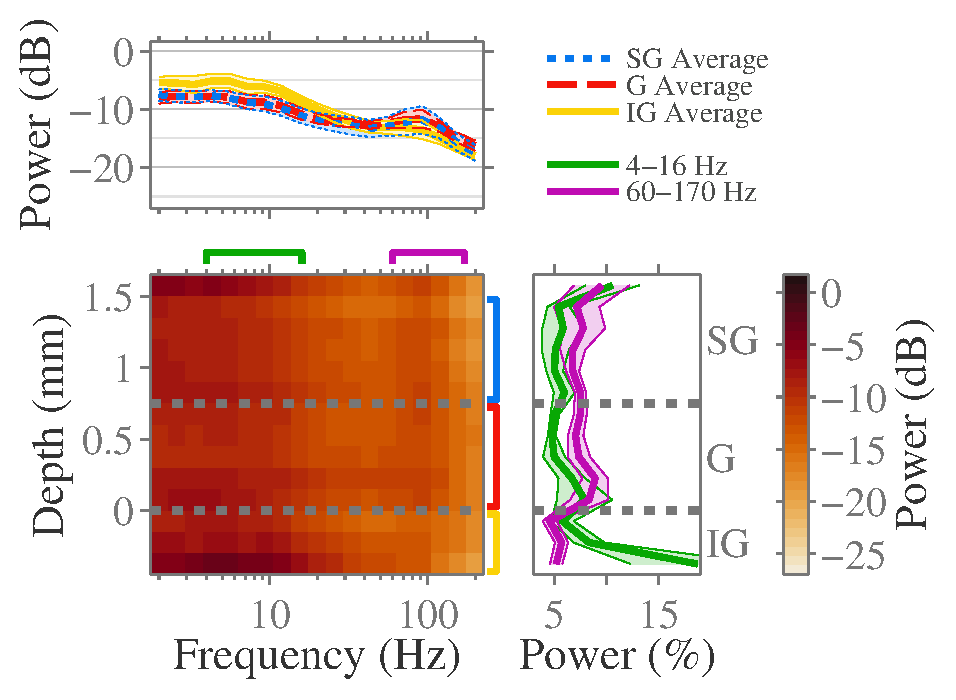
\includegraphics[scale=.45]{%
figs/info/fig3set-logRsp-Csd-power-straightnangeomean-compzonescb-legend.eps}}
    \hspace*{\fill}
    \\
    \hspace*{\fill}
    \subfloat[][\acs{LFP} information.\label{fig:lam_info_lfp}]{%
        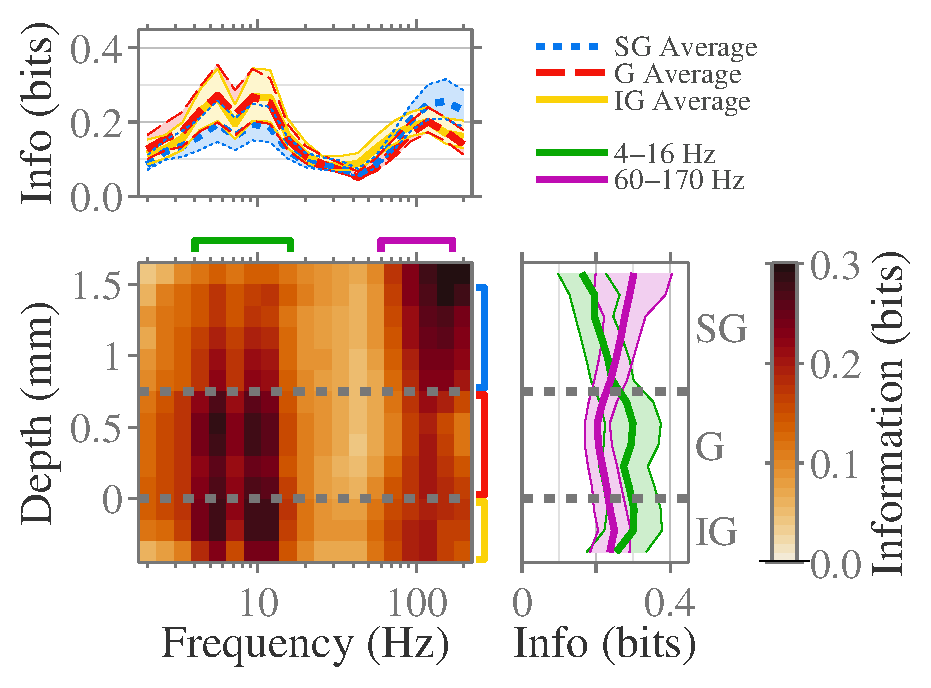
\includegraphics[scale=.45]{%
figs/info/fig3set-info-Cln-power-straightnanmean-compzonescb-legend.eps}}
    \hspace*{\fill}\hspace{.2cm}\hspace*{\fill}
    \subfloat[][\acs{CSD} information.\label{fig:lam_info_csd}]{%
        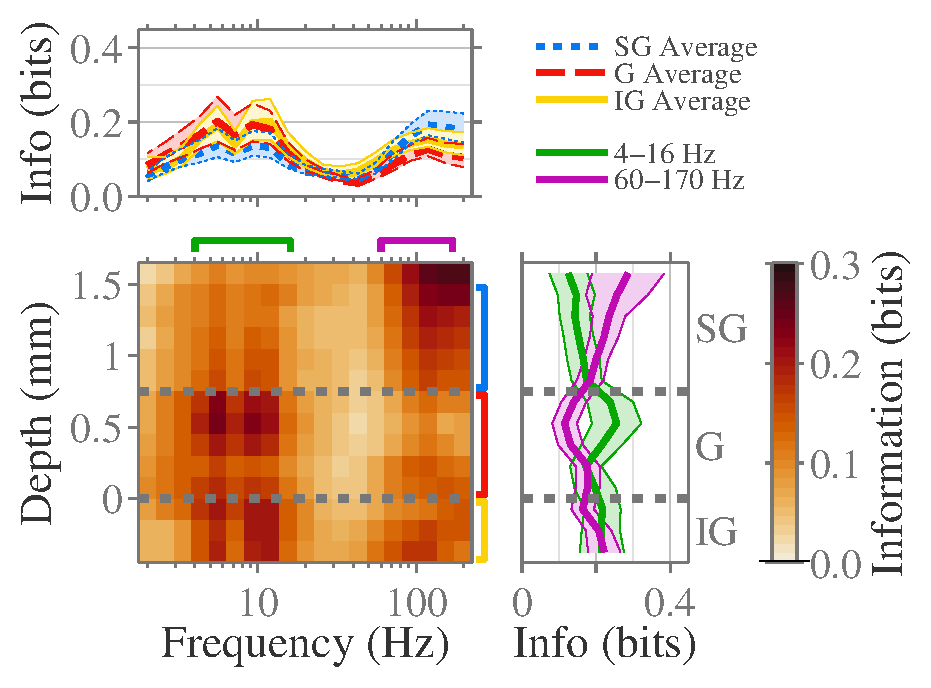
\includegraphics[scale=.45]{%
figs/info/fig3set-info-Csd-power-straightnanmean-compzonescb-legend.eps}}
    \hspace*{\fill}
    \caption{
    \textit{Distribution of visual stimulus information across both cortical depth and frequency.}
\protect\subref{fig:lam_power_lfp}: Distribution of \ac{LFP} power during stimulus presentation.
Plot shows the geometric mean power over \num{6} sessions.
Above, mean power within \ac{SG}, \ac{G} and \ac{IG} compartments.
Right, laminar distribution of \ac{LFP} power in \SIrange{4}{16}{Hz} and \SIrange{60}{170}{Hz} frequency bands.
\protect\subref{fig:lam_power_csd}: Same as \protect\subref{fig:lam_power_lfp}, but distribution of \ac{CSD} power instead of \ac{LFP} power.
\protect\subref{fig:lam_info_lfp}: Distribution of information about the stimulus contained in \ac{LFP} power.
Plot shows the mean information over \num{6} sessions.
Above, mean information within \ac{SG}, \ac{G} and \ac{IG} compartments.
Right, cortical distribution of information in the power in \SIrange{4}{16}{Hz} and \SIrange{60}{170}{Hz} frequency bands.
\protect\subref{fig:lam_info_csd}: Same as \protect\subref{fig:lam_info_lfp}, but for information in \ac{CSD} power instead of \ac{LFP} power.
Note that the information (\protect\subref{fig:lam_info_lfp} and \protect\subref{fig:lam_info_csd}) is distributed very differently from the \ac{LFP} and \ac{CSD} power (\protect\subref{fig:lam_power_lfp} and \protect\subref{fig:lam_power_csd}).
Each datapoint in \protect\subref{fig:lam_info_lfp} and \protect\subref{fig:lam_info_csd} was tested for statistical significance using bootstrapping, and each datapoint was found to be significant.
    \label{fig:lam_info}
    \label{fig:lam_2}
}
\end{figure}


We quantified these observations by computing how much information the spectral power of the \ac{LFP} and \ac{CSD} contain about the identity of which movie frame is currently on screen (see Experimental Methods).
Despite the fact that the power is distributed evenly across depth and decays smoothly as frequency increases (Figures \ref{fig:lam_power_lfp} and \ref{fig:lam_power_csd}), we found that information in the spectral power was localised around particular depths and frequencies (Figures \ref{fig:lam_info_lfp} and \ref{fig:lam_info_csd}).

For both \ac{LFP} and \ac{CSD}, information about the movie is highest in the \SIrange{4}{16}{Hz} range at the top of the granular (\ac{G}) compartment (layer 4A/B), and the \SIrange{60}{250}{Hz} range near the top of the \ac{SG} compartment (layer 2).
Additionally, there are secondary local maxima in \ac{IG} for both the \SIrange{4}{16}{Hz} and \SIrange{60}{150}{Hz} ranges.
These results are consistent across sessions (\autoref{fig:lam_s2}).
Since \ac{LFP} and \ac{CSD} have the same distribution of information, but the \ac{CSD} has better spatial localisation than the \ac{LFP} \citep{Einevoll2013,Kajikawa2011}, we will restrict ourselves to only studying the \ac{CSD} for the remainder of the paper.

These results suggest that within a single neocortical column there are two frequency bands which act as stimulus-encoding channels, which are approximately the \SIrange{4}{16}{Hz} and \SIrange{60}{170}{Hz} frequency ranges.


\subsection{Distribution of information across depth and frequency, per recording session}

The information about the stimulus contained in the power of the cortical oscillations was computed using the methodology described in the main text.
We present, in \autoref{fig:lam_s2}, the distribution of information in the power of \ac{CSD} oscillations as a function of depth and frequency for each experimental recording session.
The average over all sessions is shown in \autoref{fig:lam_s2}.
The distribution of information is broadly the same for across all sessions --- highest in granular \SIrange{4}{16}{Hz} and supragranular \SIrange{60}{170}{Hz}, little information about the stimulus encoded in the intermediary \SIrange{20}{50}{Hz} range --- indicating our findings are reliable.


\begin{figure}
% \centering 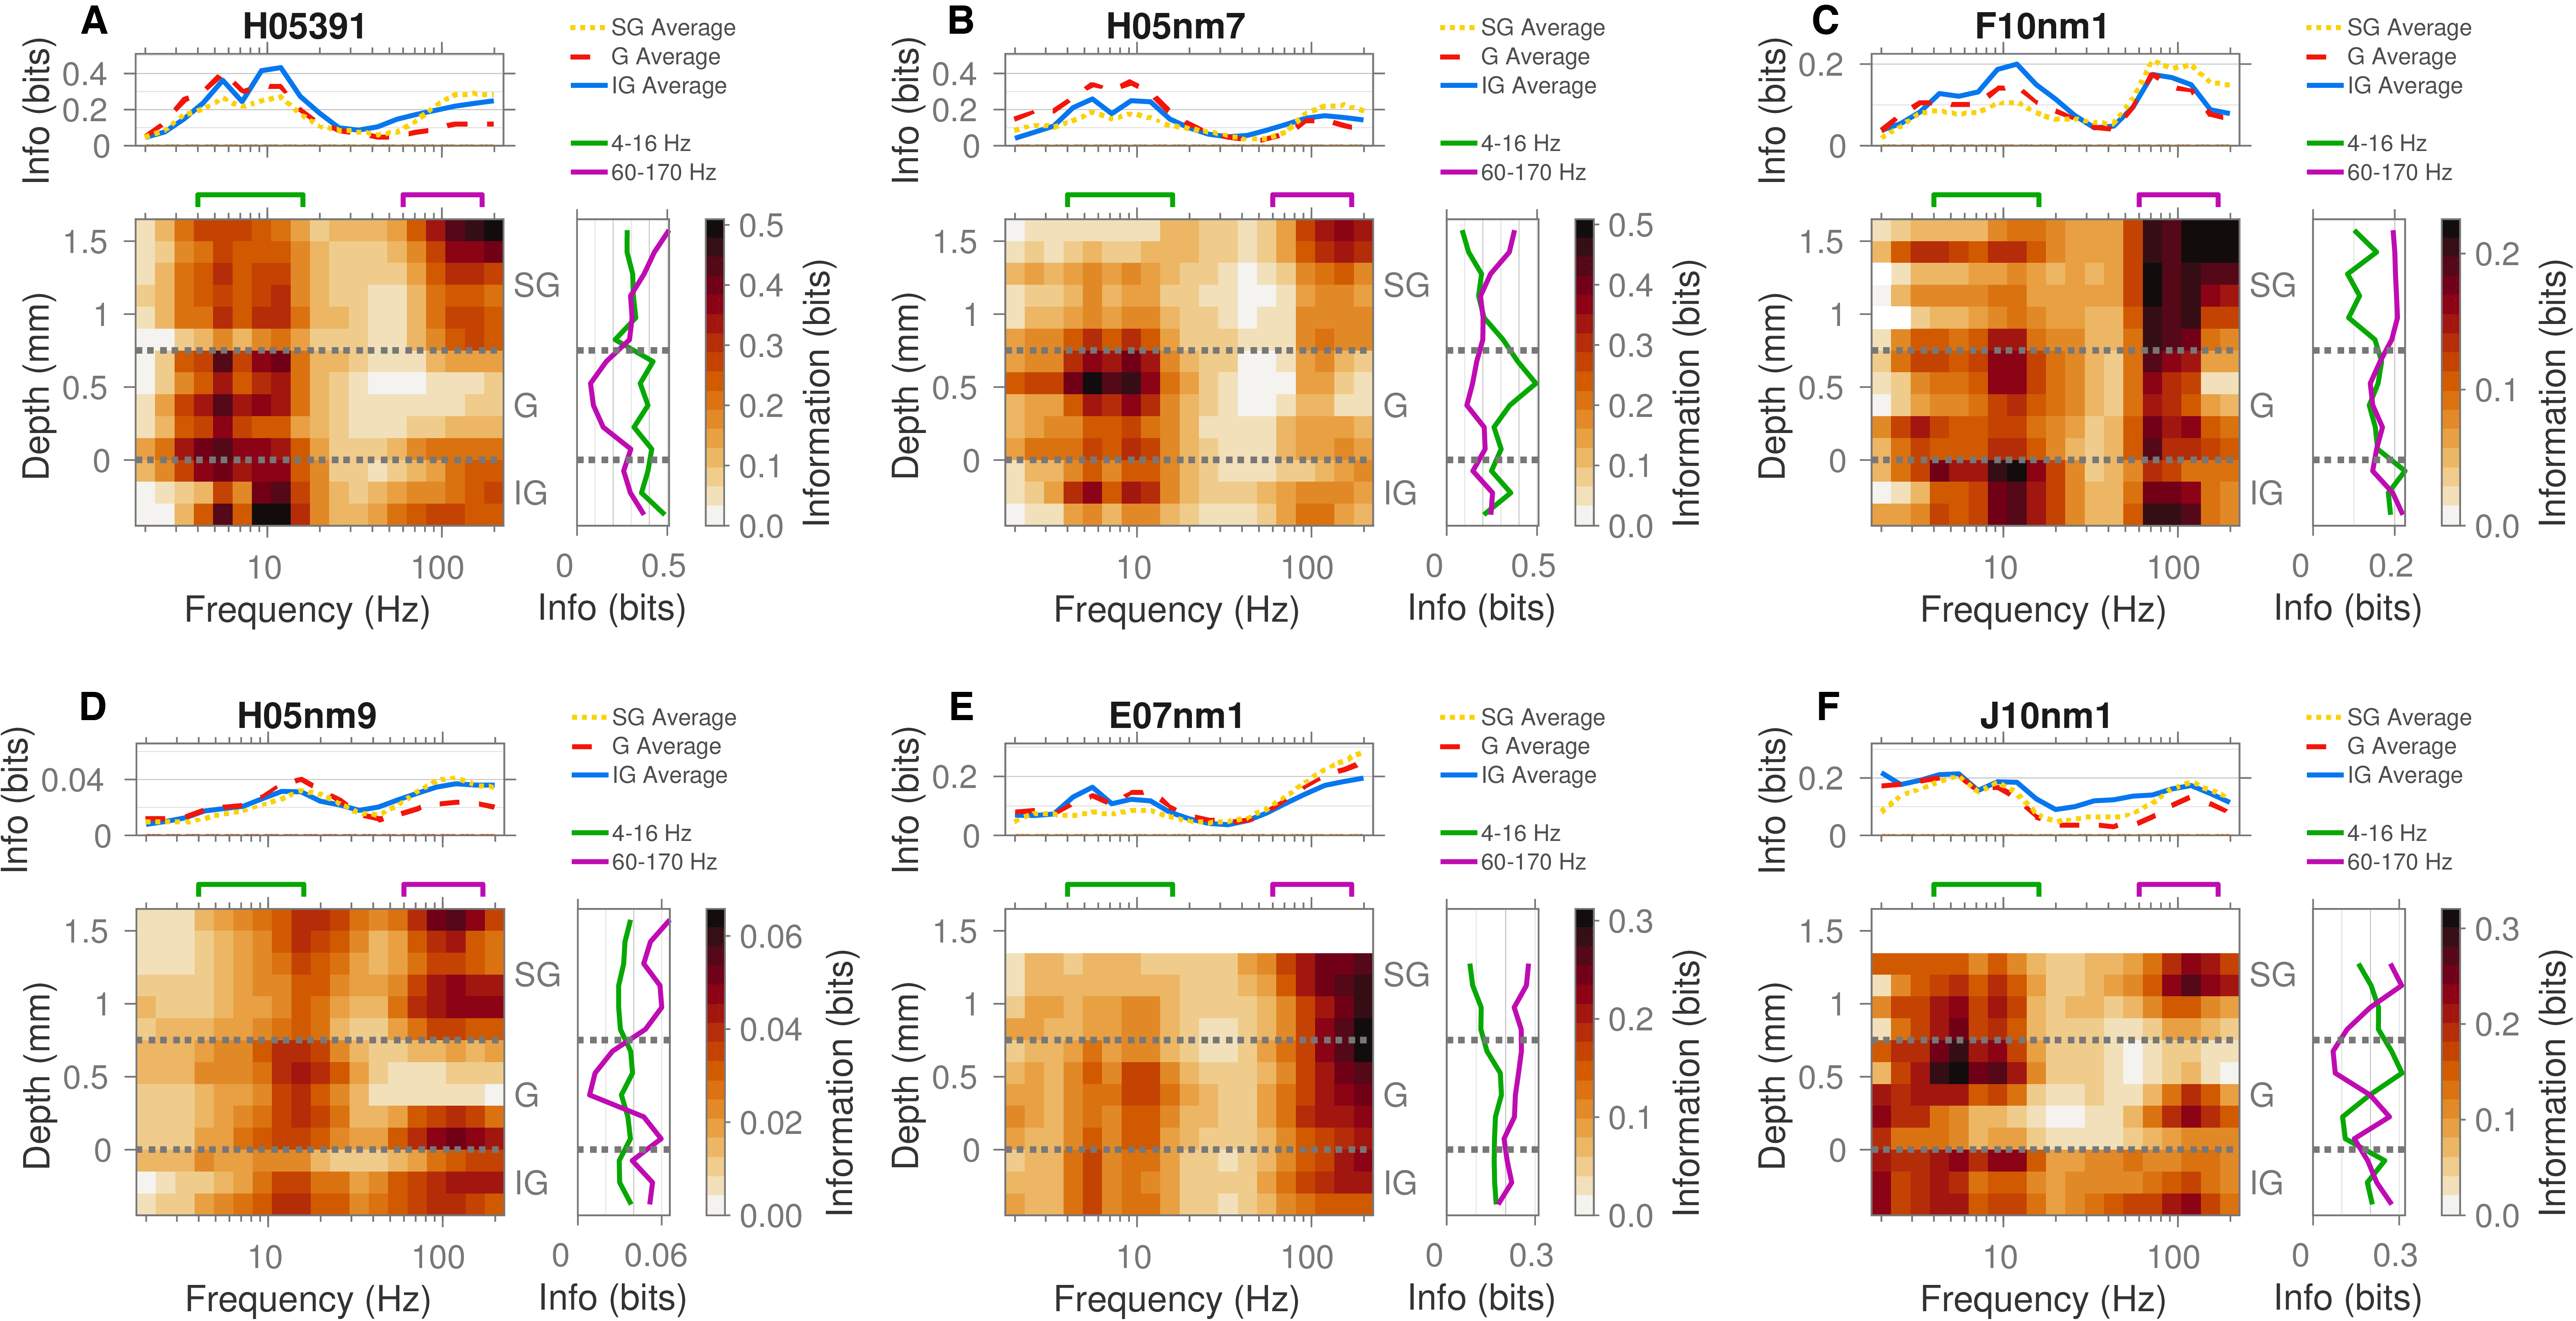
\includegraphics[width=\columnwidth]{paperfigs/figS2}
    \centering
    \hspace*{\fill}
    \subfloat[][\sesname{H05391} \acs{CSD} information.]{%
        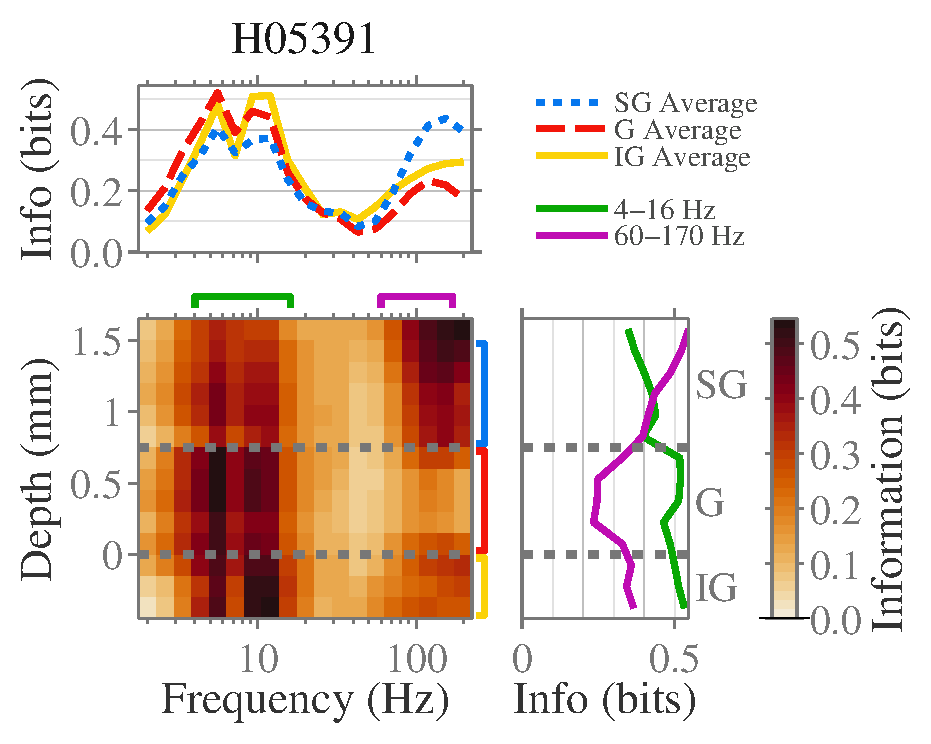
\includegraphics[scale=.45]{%
figs/info-sessions/fig3set-info-Cln-power-H05391-compzonescb-legend.eps}}
    \hspace*{\fill}\hspace{.2cm}\hspace*{\fill}
    \subfloat[][\sesname{H05nm9} \acs{CSD} information.]{%
        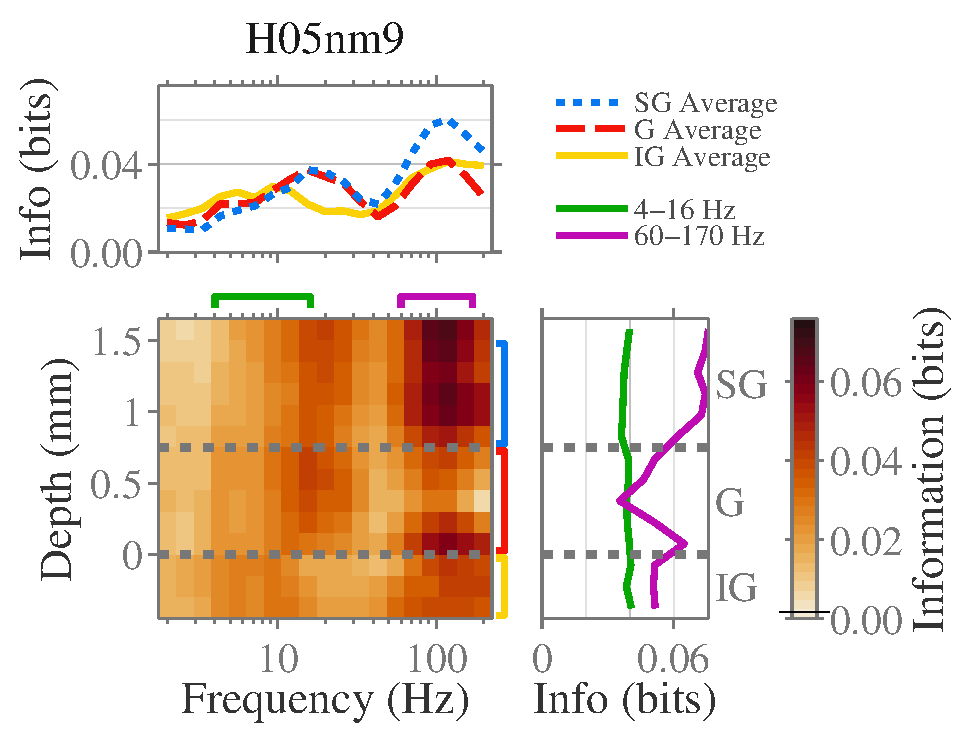
\includegraphics[scale=.45]{%
figs/info-sessions/fig3set-info-Cln-power-H05nm9-compzonescb-legend.eps}}
    \hspace*{\fill}
    \\
    \hspace*{\fill}
    \subfloat[][\sesname{H05nm7} \acs{CSD} information.]{%
        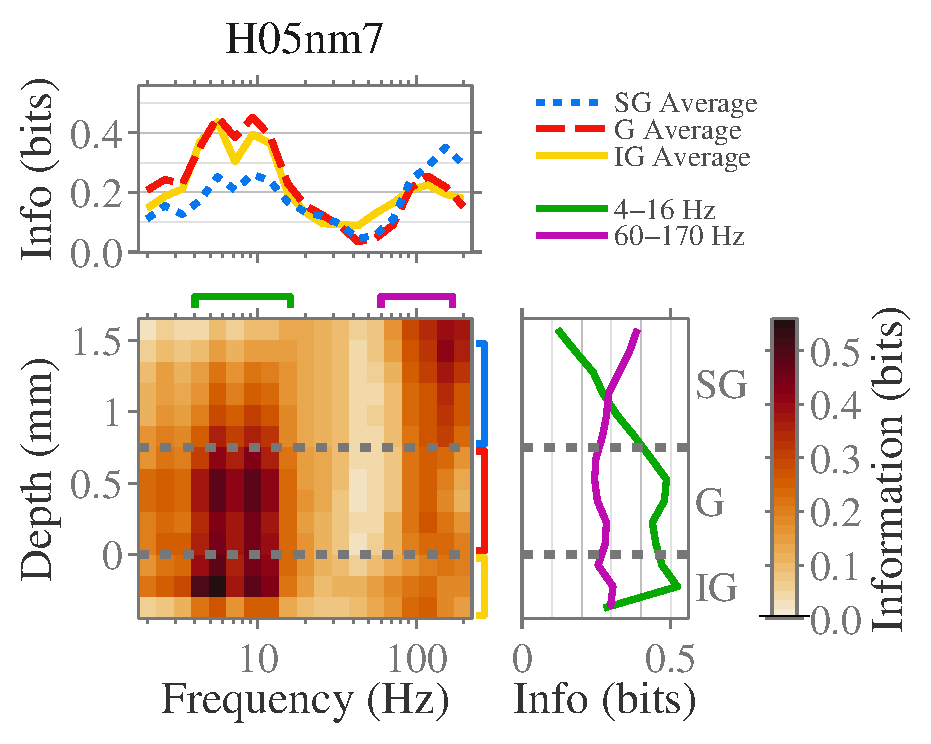
\includegraphics[scale=.45]{%
figs/info-sessions/fig3set-info-Cln-power-H05nm7-compzonescb-legend.eps}}
    \hspace*{\fill}\hspace{.2cm}\hspace*{\fill}
    \subfloat[][\sesname{E07nm1} \acs{CSD} information.]{%
        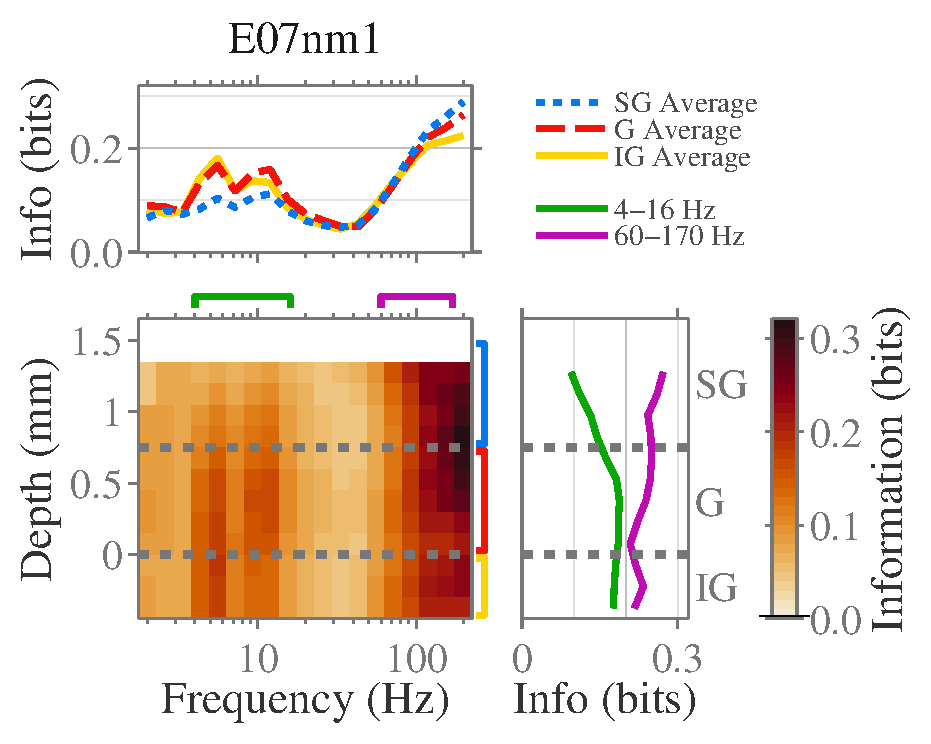
\includegraphics[scale=.45]{%
figs/info-sessions/fig3set-info-Cln-power-E07nm1-compzonescb-legend.eps}}
    \hspace*{\fill}
    \\
    \hspace*{\fill}
    \subfloat[][\sesname{F10nm1} \acs{CSD} information.]{%
        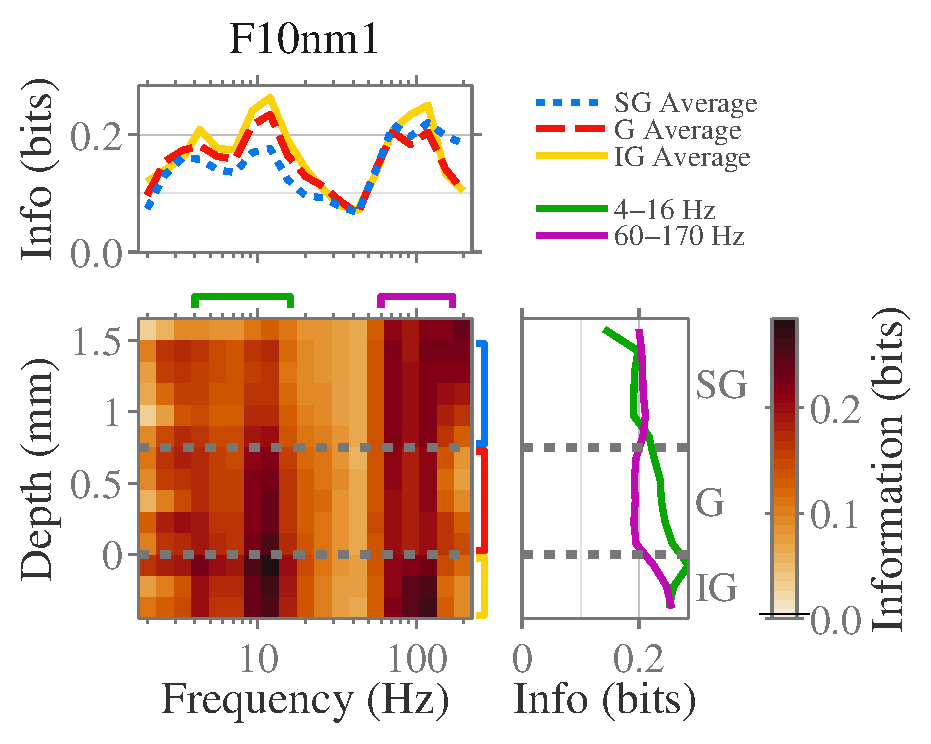
\includegraphics[scale=.45]{%
figs/info-sessions/fig3set-info-Cln-power-F10nm1-compzonescb-legend.eps}}
    \hspace*{\fill}\hspace{.2cm}\hspace*{\fill}
    \subfloat[][\sesname{J10nm1} \acs{CSD} information.]{%
        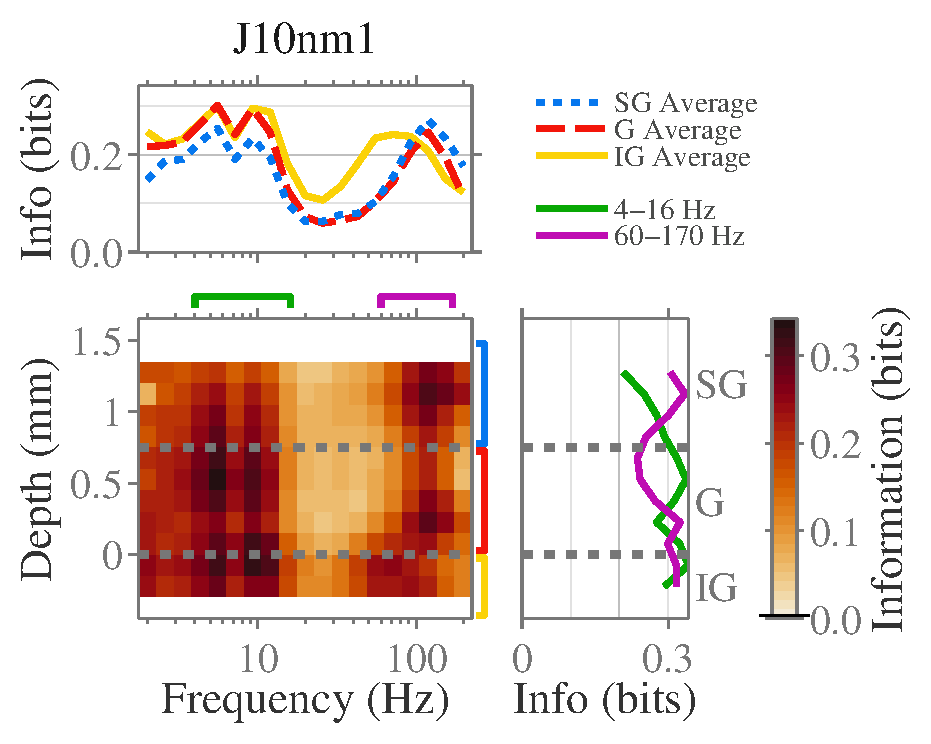
\includegraphics[scale=.45]{%
figs/info-sessions/fig3set-info-Cln-power-J10nm1-compzonescb-legend.eps}}
    \hspace*{\fill}
%
\caption{%
\textit{Distribution of information about the movie across both cortical depth and frequency for individual sessions}
Same as \autoref{fig:lam_info_csd}, but shown for each recording session individually.
}
\label{fig:lam_s2}
%
\end{figure}


\subsection{Information redundancy between frequencies}
However, these results raise the question whether the two frequency ranges encode the same or different information about the stimulus, and whether the same information is encoded within a given frequency band across the entire cortical depth. 
To answer this we computed the redundancy between pairs of frequency bands of the information about the stimulus which they encode (see Experimental Methods).
Computing information redundancy allows us to quantify how similar the information about the stimulus is for a given pair of frequency bands and depths --- high redundancy shows the information about the stimulus is mostly the same in the two bands, low redundancy means the two bands contain independent information about the stimulus (see Experimental Methods for a formal definition).
We found there are two frequency domains within which information is redundant: \SIrange{4}{40}{Hz} and \SI{>40}{Hz} (\autoref{fig:lam_3}A).
Furthermore, the information contained in neural frequencies \SI{<40}{Hz} is different to the information contained in frequencies \SI{>40}{Hz}, since these measured to be independent (redundancy \SI{<=0}{\percent}).
Additionally, we note that the same \SI{<40}{Hz} and \SI{>40}{Hz} division is observed for the signal correlation (\autoref{fig:lam_s3}), and our results corroborate earlier findings \citep{Belitski2008}.
These results thus show that the two bands (\SIrange{4}{16}{Hz} and \SIrange{60}{170}{Hz}) contain the most information and independently encode information about the stimulus.

\begin{figure}[htbp]
\centering 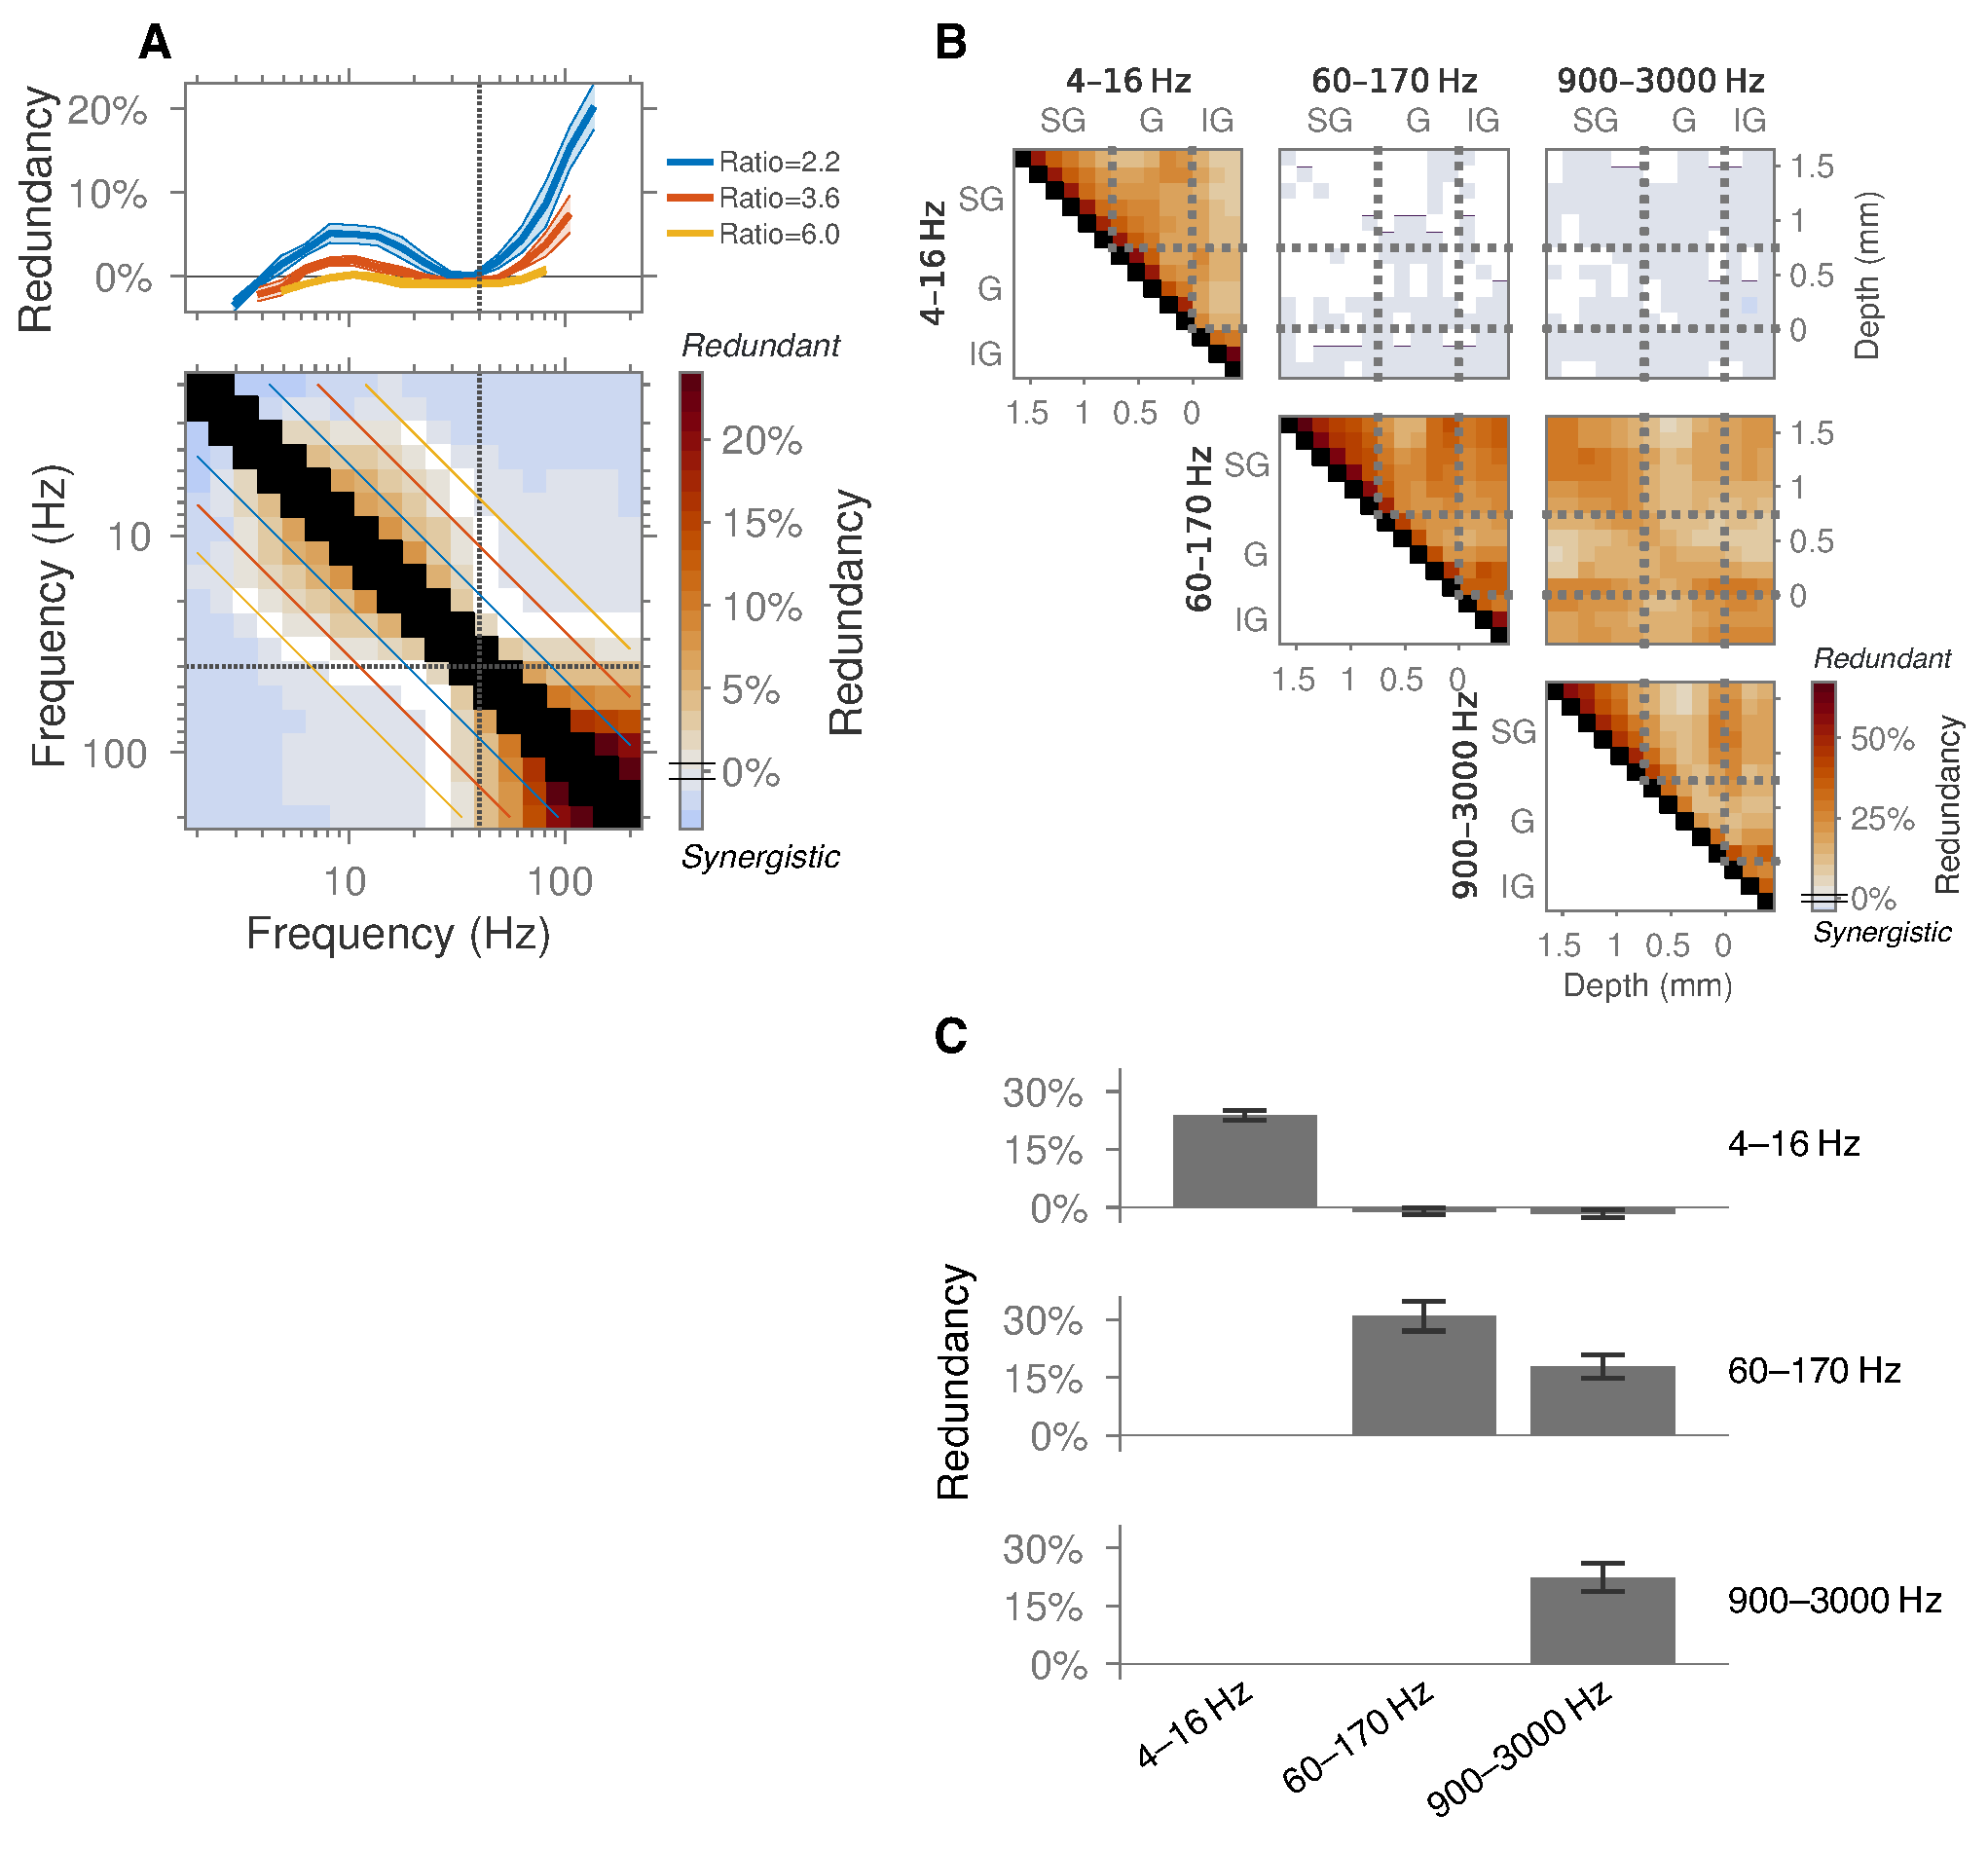
\includegraphics[width=\columnwidth]{paperfigs/fig3}
%
\caption{%
\textit{Information redundancy across frequency bands and laminae in the CSD signal.}
A: Median redundancy between pairs of frequencies over the \num{12} recording sites, averaged over \num{6} sessions.
B: Redundancy between pairs of recording sites of the information in three frequency bands. Mean of \num{6} sessions.
C: Average of cross-channel redundancy shown in B.
In A and B, datapoints which were not significantly different from $0$ (threshold at \num{3} standard deviations of bootstrapped information values) are shown in white.
In C, error bars indicate \num{3} standard deviations of the bootstrapped values after averaging.
Trivially redundant diagonal elements were removed.
Note, that while there is substantial redundancy within bands and between the \SIrange{60}{170}{Hz} and \SIrange{900}{3000}{Hz} bands, there is little redundancy between the \SIrange{4}{16}{Hz} and \SIrange{60}{170}{Hz} band, indicating independent coding.
}%
\label{fig:lam_3}
%
\end{figure}


\subsection{Information redundancy across depth}

Next, we investigated whether the information contained in these frequency bands was the same across the cortical depths.
To this end, we computed the redundancy of the information about the stimulus contained in oscillations at different cortical depths, both within the same band at each depth, and between different bands (\autoref{fig:lam_3}B; see Experimental Methods).

Within the \SIrange{4}{16}{Hz} frequency range, there is redundancy across the entire cortical depth, but there are two distinct cortical compartments (above and below the \ac{CSD} reversal, marked as \SI{0}{mm} depth) within which there is increased redundancy.
These findings are in agreement with \citet{Maier2010}, who found a transition corresponding to the \ac{G}/\ac{IG} boundary which isolated two cortical compartments with high coherence \SI{<100}{Hz}.
Gamma oscillations (\SIrange{60}{170}{Hz}) have substantial redundancy across the cortical depth.

We also compared this to spiking activity by analysing the  \SIrange{900}{3000}{Hz} frequency range, whose power corresponds to \ac{MUA}. The information in this  band is redundant with the \SIrange{60}{170}{Hz} frequency band.
This indicates that the population spiking activity contains the same information as the gamma range, which is in agreement with previous findings \citep{Belitski2008}.
% This is to be expected, since \ac{MUA} is known to be correlated with the gamma cycle.(due to peaks/troughs in gamma relating to peaks/troughs in firing rate).

The overall redundancy between these bands, averaged over all cortical depths emphasises these results (see \autoref{fig:lam_3}C).

[Note occasional shift  to present tense]
Comparing the \SIrange{4}{16}{Hz} band with either higher frequency bands, we found the lower frequency range contains information which is not expressed in the higher frequencies at any cortical depth.
It consequently follows that the two localised regions of high information content from \autoref{fig:lam_info_csd} (granular \SIrange{4}{16}{Hz} and supragranular \SI{>60}{Hz}) are not redundant to each other and contain complementary information about the stimulus.
%Importantly, this argues against a situation where \ac{SG} contains the same information as \ac{G}/\ac{IG} activity transcoded from low-frequency to high-gamma oscillations; at least some of the information is unique to each.

This, of course, begs the question which orthogonal properties of the stimulus could be encoded into these two complementary spectral bands.


\subsection{Noise and signal correlations}

To accompany the information redundancy between frequencies and depths (\autoref{fig:lam_s3}), we also computed the noise and signal correlation between the power of oscillations (\autoref{fig:lam_s3}).

Both the signal and noise correlation show the same pattern across frequencies (\autoref{fig:lam_s3}A and D) as the information redundancy (\autoref{fig:lam_3}A), and similarly for the distribution across depth (\autoref{fig:lam_s3}B and E; \autoref{fig:lam_3}B).
However, the relationship is less clear for the signal and noise correlation than we observed for information redundancy.
For instance, since all signals are positively correlated in \autoref{fig:lam_s3}A (and D), the difference in correlation either side of the \SI{40}{Hz} line is less clear, though still evident.


\begin{figure}
\centering 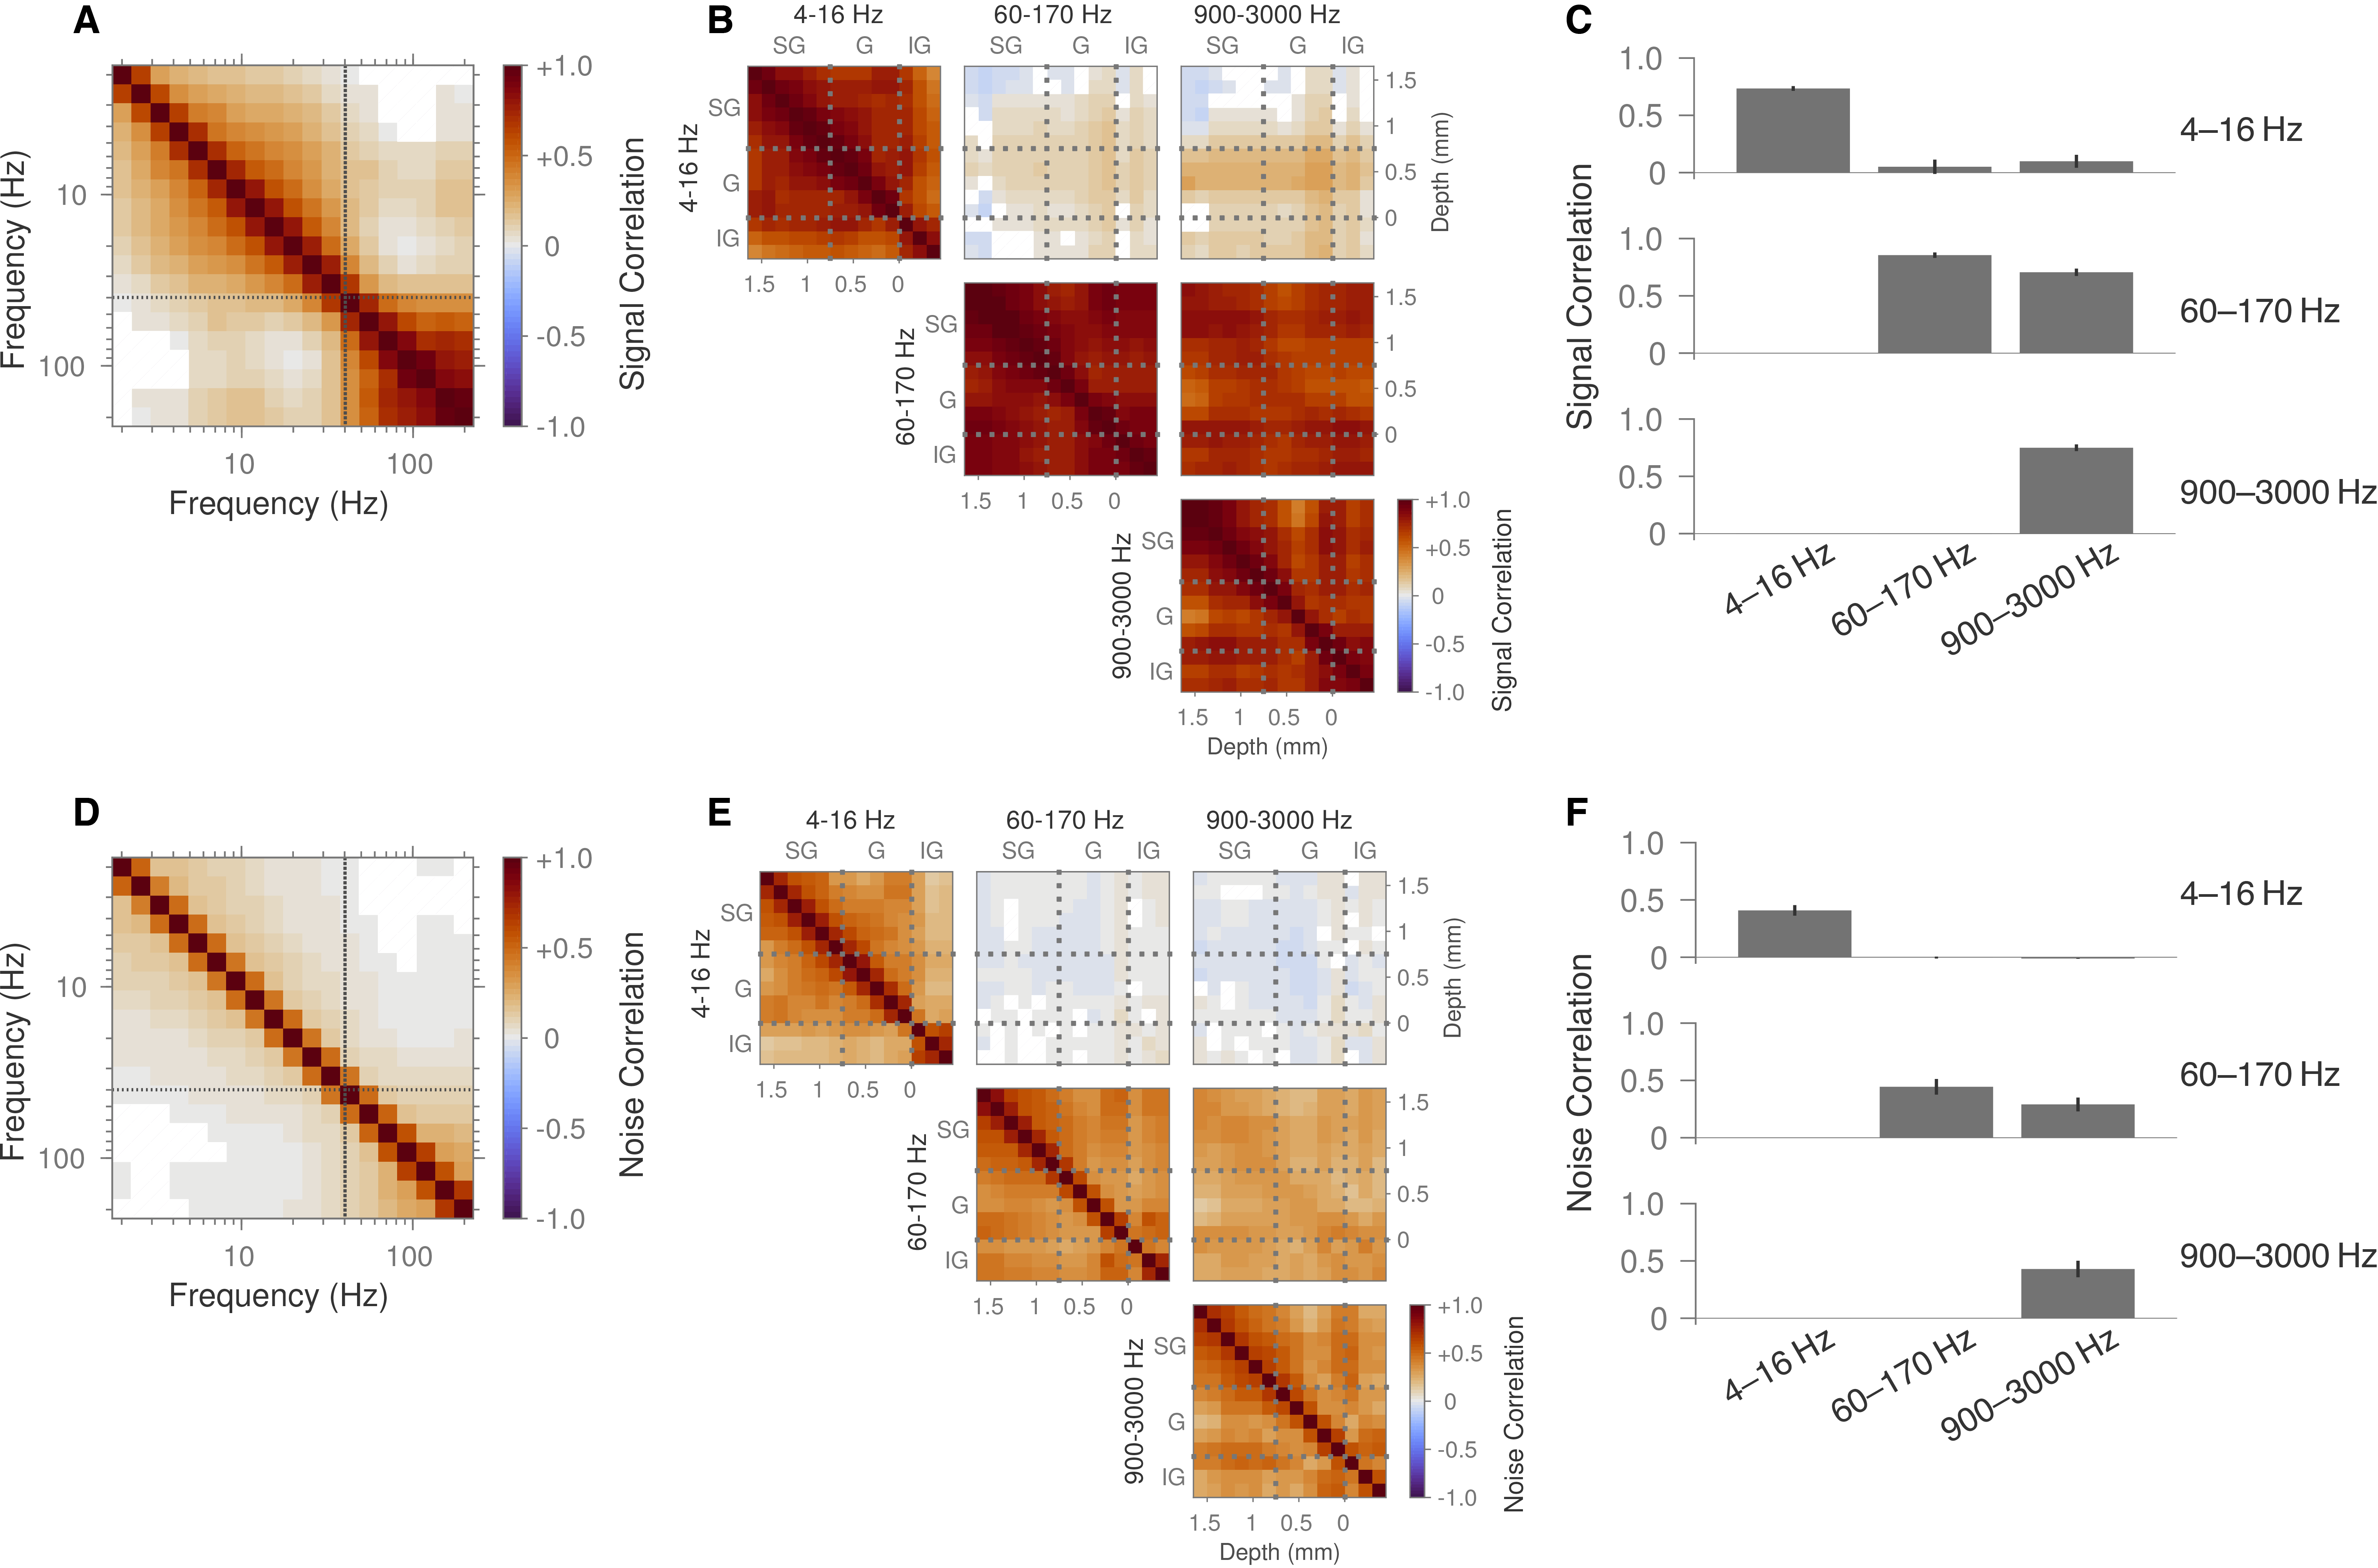
\includegraphics[width=\columnwidth]{paperfigs/figS3}
%
\caption{%
\textit{Signal and noise correlations.}
A: Median signal correlation between pairs of frequencies of the 14 recording sites, mean across 6 sessions.
Above, traces along the off-diagonals of the heatmap.
Each trace shows the redundancy between two bands with fixed ratio between their frequencies, against their geometric mean, with the shaded region indicating the standard error on the mean over 6 sessions.
B: Same as A, except for noise correlation instead of signal correlation.
C: Signal correlation between pairs of recording sites across the three frequency bands.
Mean of 6 sessions.
D: As C, but showing noise correlation.
E: Average signal correlation between each pair of frequency bands, found by averaging over all pairs of electrode contacts (excluding the trivial same-depth auto-correlation).
Error bars indicate the standard error over the 6 sessions.
F: As E, but showing noise correlation.
In A--D, datapoints which were not significantly different from the bootstrap mean (threshold at 3 standard deviations of bootstrapped correlation values) are shown in white.
The maximum upper and minimum lower thresholds employed for significance are shown on the colour bars.
Trivially correlated diagonal elements were removed (shown in black).
}
\label{fig:lam_s3}
%
\end{figure}


\subsection{Information about spatial frequency components of visual stimulus}

Above, we have demonstrated that there are two frequency bands in \ac{V1} which, across all the cortical depth, contain independent information to each other.
Since neurons in the primary visual cortex are known to respond strongly to moving sinusoidal gratings with specific spatial frequencies, we investigated how much information the frequency bands contained about changes in luminance as a function of spatial frequency.
We decomposed the series of frames in the movie into set of spatial frequency components by finding the rate of change of luminance within a given set of spatial frequency bands (see \autoref{fig:lam_4}; Experimental Methods), and then computed the amount of information about this series contained in the neural activity.

\begin{figure}[htbp]
\centering 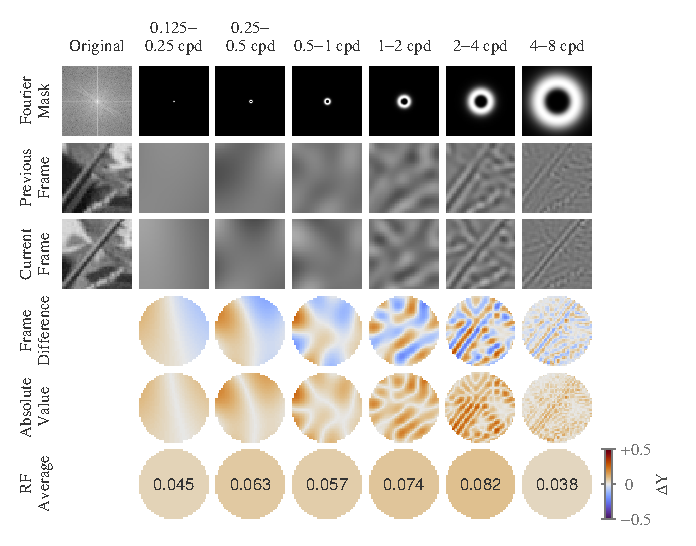
\includegraphics[width=\columnwidth]{paperfigs/fig4}
%
\caption{%
\textit{Extraction of spatially filtered luminance components.}
The luminance of the original video (left) is fast-Fourier transformed in a \SI{224x224}{px} square for each frame (top-left: \ac{FFT} of  ``current frame'').
The mask isolates bands of spatial frequencies that are one octave wide (Row 1), yielding the spatially filtered frames (Rows 2 and 3).
The stimulus magnitude at each spatial frequency band was obtained by taking the luminance difference of successive frames (Row 4), taking its absolute value (Row 5), and averaging this within the receptive field (Row 6). [remove discs in Row6 ]
%This provides us with a temporal sequence of the rate of change of luminance for 
%each spatial resolution.
}%
\label{fig:lam_4}
%
\end{figure}

\begin{figure}[htbp]
\centering 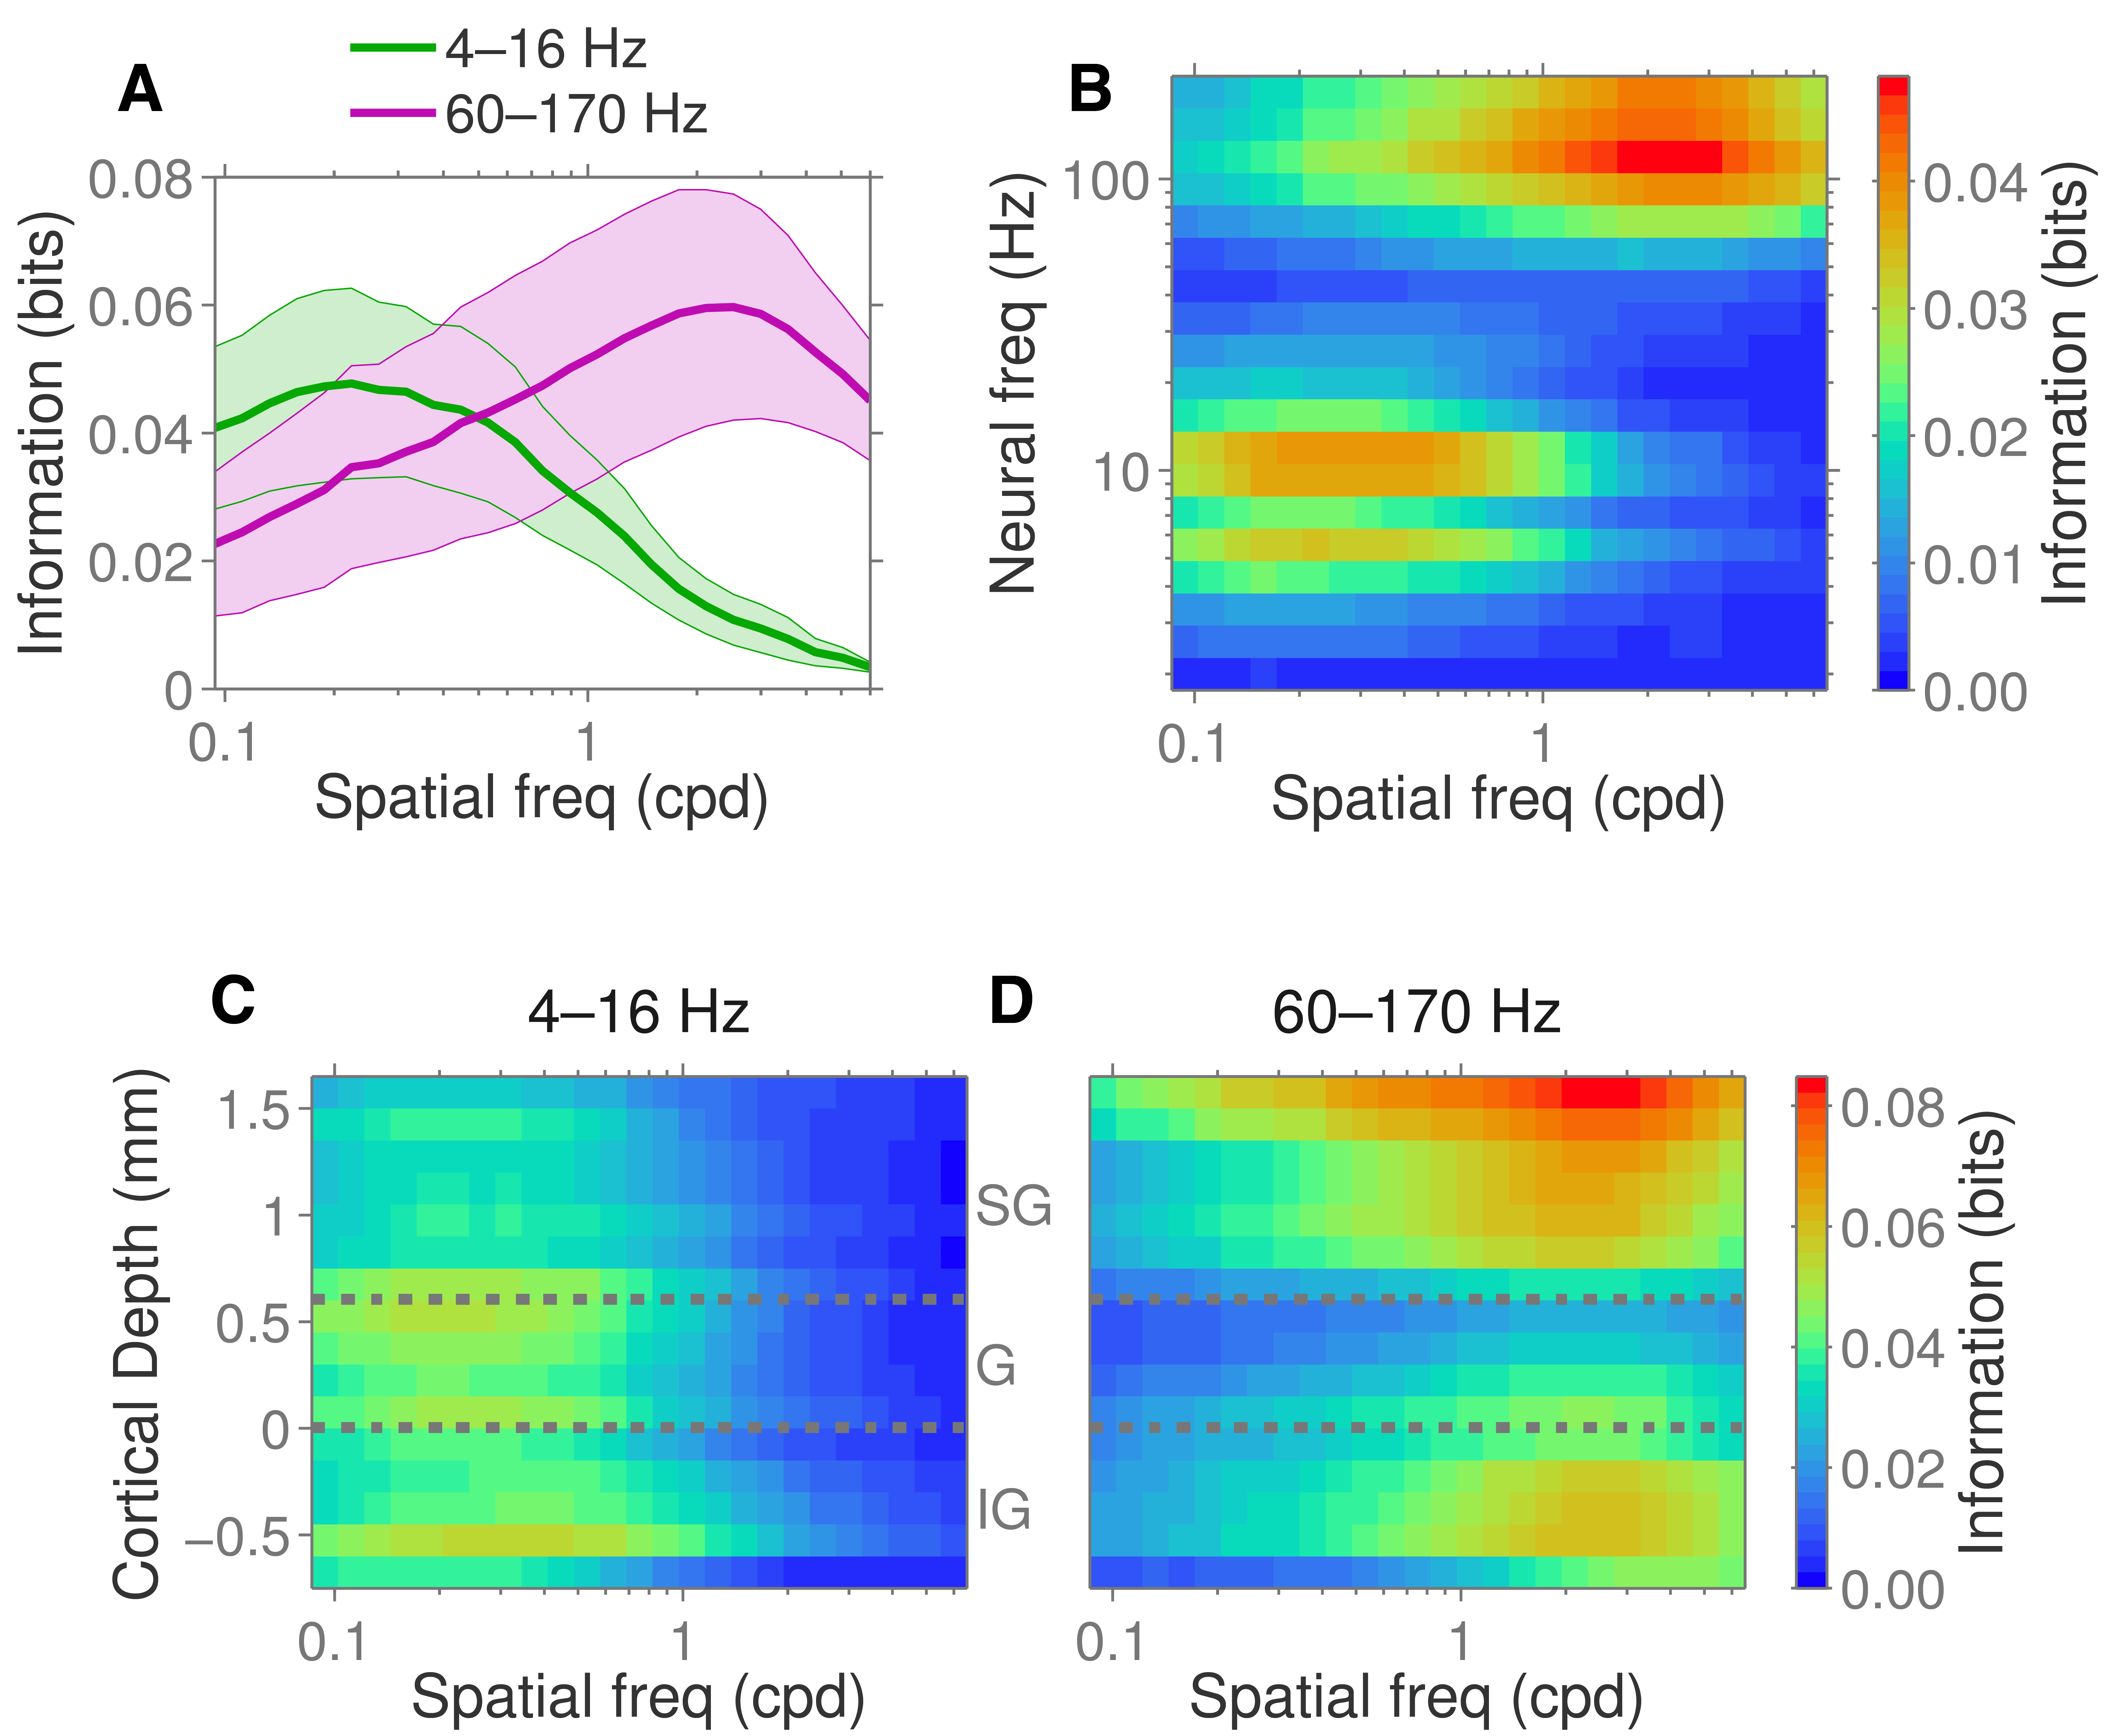
\includegraphics[width=\columnwidth]{paperfigs/fig5}
%
\caption{%
\textit{Information about different spatial components across laminae and frequency bands.}
A: Information about spatial components of the stimulus contained in low frequency \ac{CSD} power (\SIrange{4}{16}{Hz}, average of information within \ac{G} compartment; green) and high frequency \ac{CSD} power (\SIrange{60}{170}{Hz}, average of information within \ac{SG} compartment; purple).
Shaded area: standard error across \num{6} sessions.
B: Information about visual spatial components contained in a range of \ac{CSD} frequencies, median over \num{12} recording sites.
C,D: Information in low (\SIrange{4}{16}{Hz}) and high (\SIrange{60}{170}{Hz}) \ac{CSD} frequency bands across cortical laminae.
Plots A-D are mean of \num{6} sessions.}%
\label{fig:lam_5}
%
\end{figure}
The results are summarised in \autoref{fig:lam_5}A, which shows the information encoded in these two frequency bands, averaged across the whole cortical depth.
We found the low frequency \ac{CSD} bands (\SI{<40}{Hz}) contained more information about low spatial frequencies (\SIrange{0.1}{0.6}{\cpd}), whereas the higher spectral frequencies (\SI{>40}{Hz}) contained more information about high spatial frequencies (\SIrange{0.6}{5.0}{\cpd}) (\autoref{fig:lam_5}B).
Importantly, there was no continuous transition between these two; instead we observe an abrupt change at \SI{40}{Hz}, with lower and higher neural oscillation frequencies tuned to stimulus features with different spatial frequencies.
Neural oscillations at intermediate frequencies do not encode intermediate spatial components of the stimulus --- they do not encode any spatial aspect of the stimulus.

These observations held true across the entire cortical depth (\autoref{fig:lam_5}C--D), with the two frequency bands (\SIrange{4}{16}{Hz} and \SIrange{60}{170}{Hz}) containing information about opposing spatial frequencies.
The distribution of information across the cortical depth corresponds to that found in \autoref{fig:lam_info_csd}.

Since information theoretic measures capture any possible relationship between stimulus and response, we cannot use it to determine the nature of how changes in luminance lead to changes .in cortical power.
To resolve this question, we investigated the correlation between the \ac{CSD} power and both coarse (\SI{<0.3}{\cpd}, low-pass spatial filter) and fine (\SI{>1}{\cpd}, high-pass spatial filter) spatial components of the movie stimulus, illustrative example traces of which are shown above \autoref{fig:lam_6}A.
These spatial components have a low coefficient of correlation with each other (\autoref{fig:lam_6}B; $r=0.18$), indicating these two aspects of the movie stimulus do not notably co-vary with each other.

We found (\autoref{fig:lam_6}A) the low frequency \ac{CSD} power is positively correlated with the coarse changes in luminance, and high frequency \ac{CSD} power is positively correlated with the finer changes in luminance --- in both cases an increase in luminance of the stimulus yields an increase in power as a response.

Example \ac{CSD} traces are shown for two electrode contacts (\autoref{fig:lam_6}A, left side) over same time period as the luminance example traces.
By visual inspection, one can observe that peaks and troughs in the luminance signals are coincident with peaks and troughs \ac{CSD} power of the appropriate frequency range.
[1. Information in fig 6A remain undiscussed. 2 Was correlation also calculated at optimal lag?]

\begin{figure}[htbp]
\centering 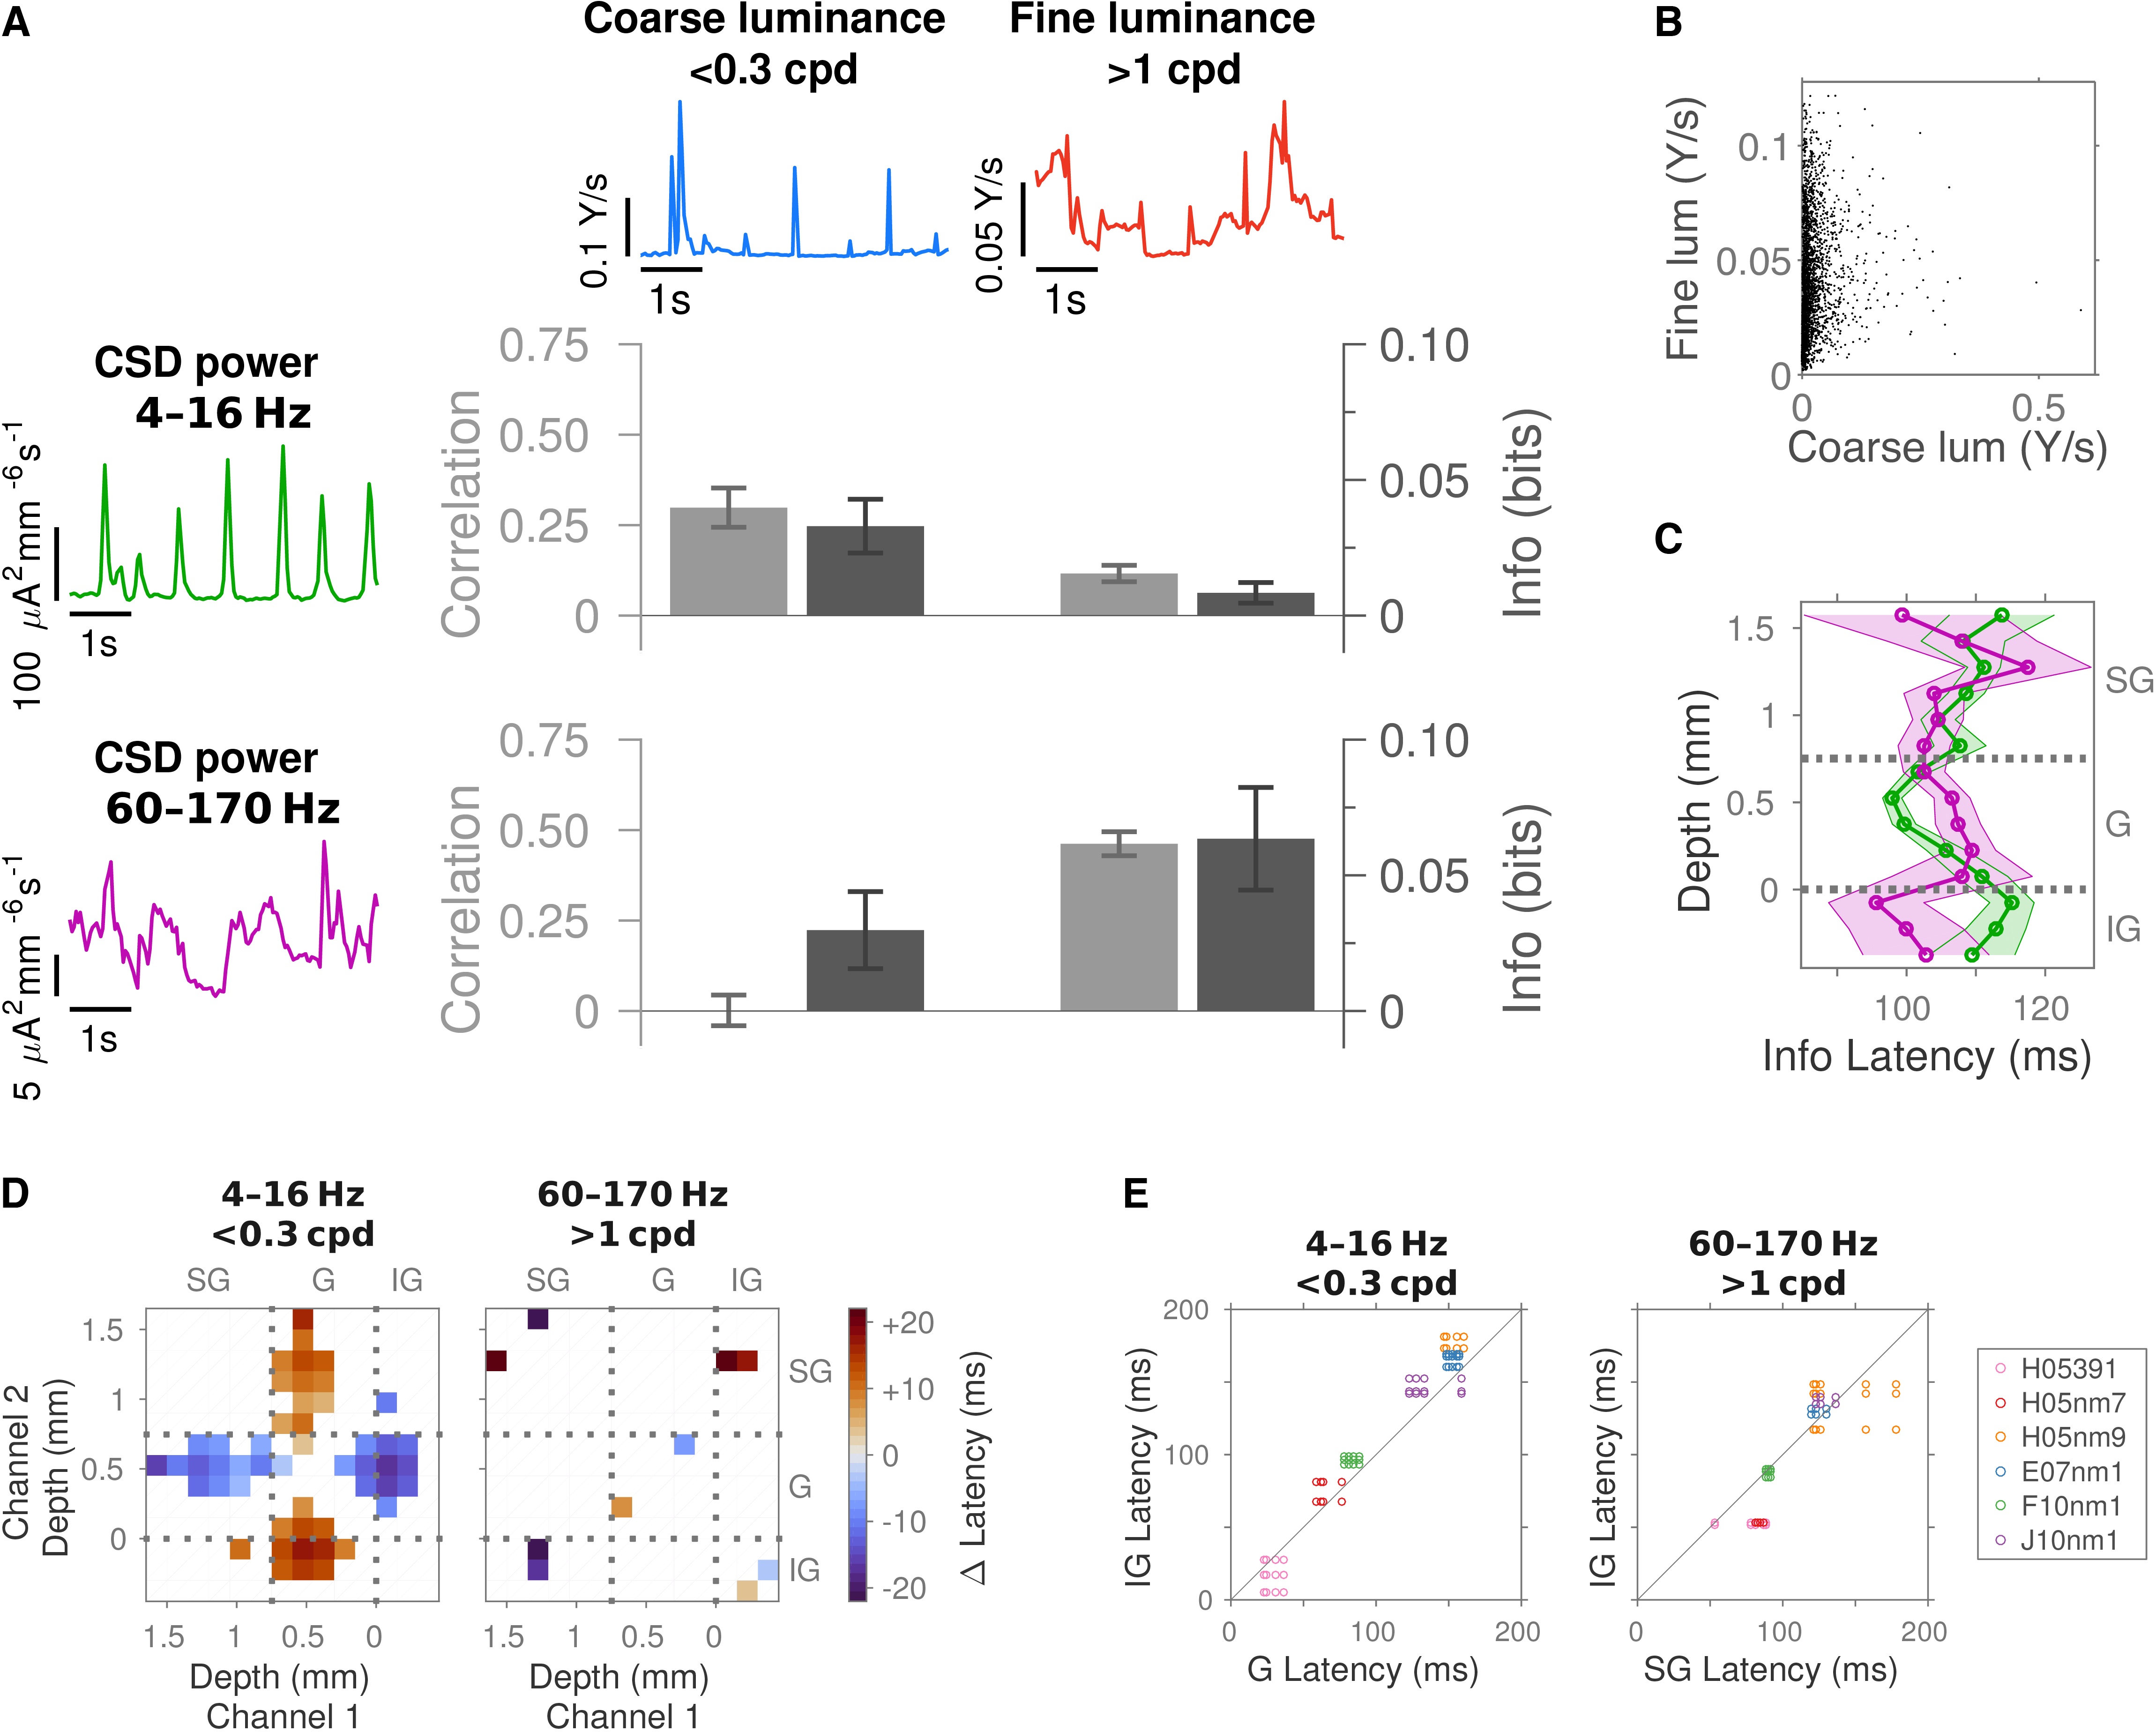
\includegraphics[width=\columnwidth]{paperfigs/fig6}
%
\caption{%
\textit{Overview of information components.}
A: Relationship between Coarse/Fine changes in luminance and Low/High frequency neural activity.
Left: Instantaneous power in \SIrange{4}{16}{Hz} band (averaged over trials and \ac{SG} layers) and \SIrange{60}{170}{Hz} band (averaged over trials and \ac{G} layers) for an example session (\sesname{H05nm7}).
Above: Coarse (\SI{<0.3}{\cpd}) and fine (\SI{>1}{\cpd}) rate of change in luminance over the same time period.
The barchart shows, for each pair of stimulus and response, Pearson's correlation coefficient (pale grey; left-hand axis) and mutual information (dark grey; right-hand axis).
B: Fine versus coarse change in luminance for each frame change in the stimulus.
C: Lag between stimulus and response yielding maximal information (green: \SIrange{4}{16}{Hz} and coarse luminance; purple: \SIrange{60}{170}{Hz} and fine luminance).}%
\label{fig:lam_6}
%
\end{figure}


\subsection{Layer 1 60--\SI{170}{Hz} amplitude is coupled to L5 4--\SI{16}{Hz} phase}

Above, in section ``Information redundancy across depth'', we showed that high and low \ac{CSD} frequencies contain independent information to each other (\autoref{fig:lam_3}).
We found the power in the two bands to be independent, but it remains possible that there is a relationship between the phase of the low-frequency band and the power of the high-frequency band.
To investigate this possibility, we examined the cross-frequency coupling between the low-frequency phase and high-frequency oscillation amplitude.

Our observations showed that there is a spatially localised coupling between the \SIrange{4}{16}{Hz} phase of both lower-\ac{G} and mid-\ac{IG} with the amplitude of \SIrange{60}{170}{Hz} oscillations in upper-\ac{SG} (\autoref{fig:lam_8}).
Additionally, in both \ac{G} and \ac{IG} there is a coupling between the local \SIrange{4}{16}{Hz} phase and the local \SIrange{60}{170}{Hz} amplitude.

The same relationship was discovered to hold both for spontaneous activity and stimulus-driven recordings, and our findings are in agreement with previous work \citep{Spaak2012}.

\begin{figure}[htbp]
\centering 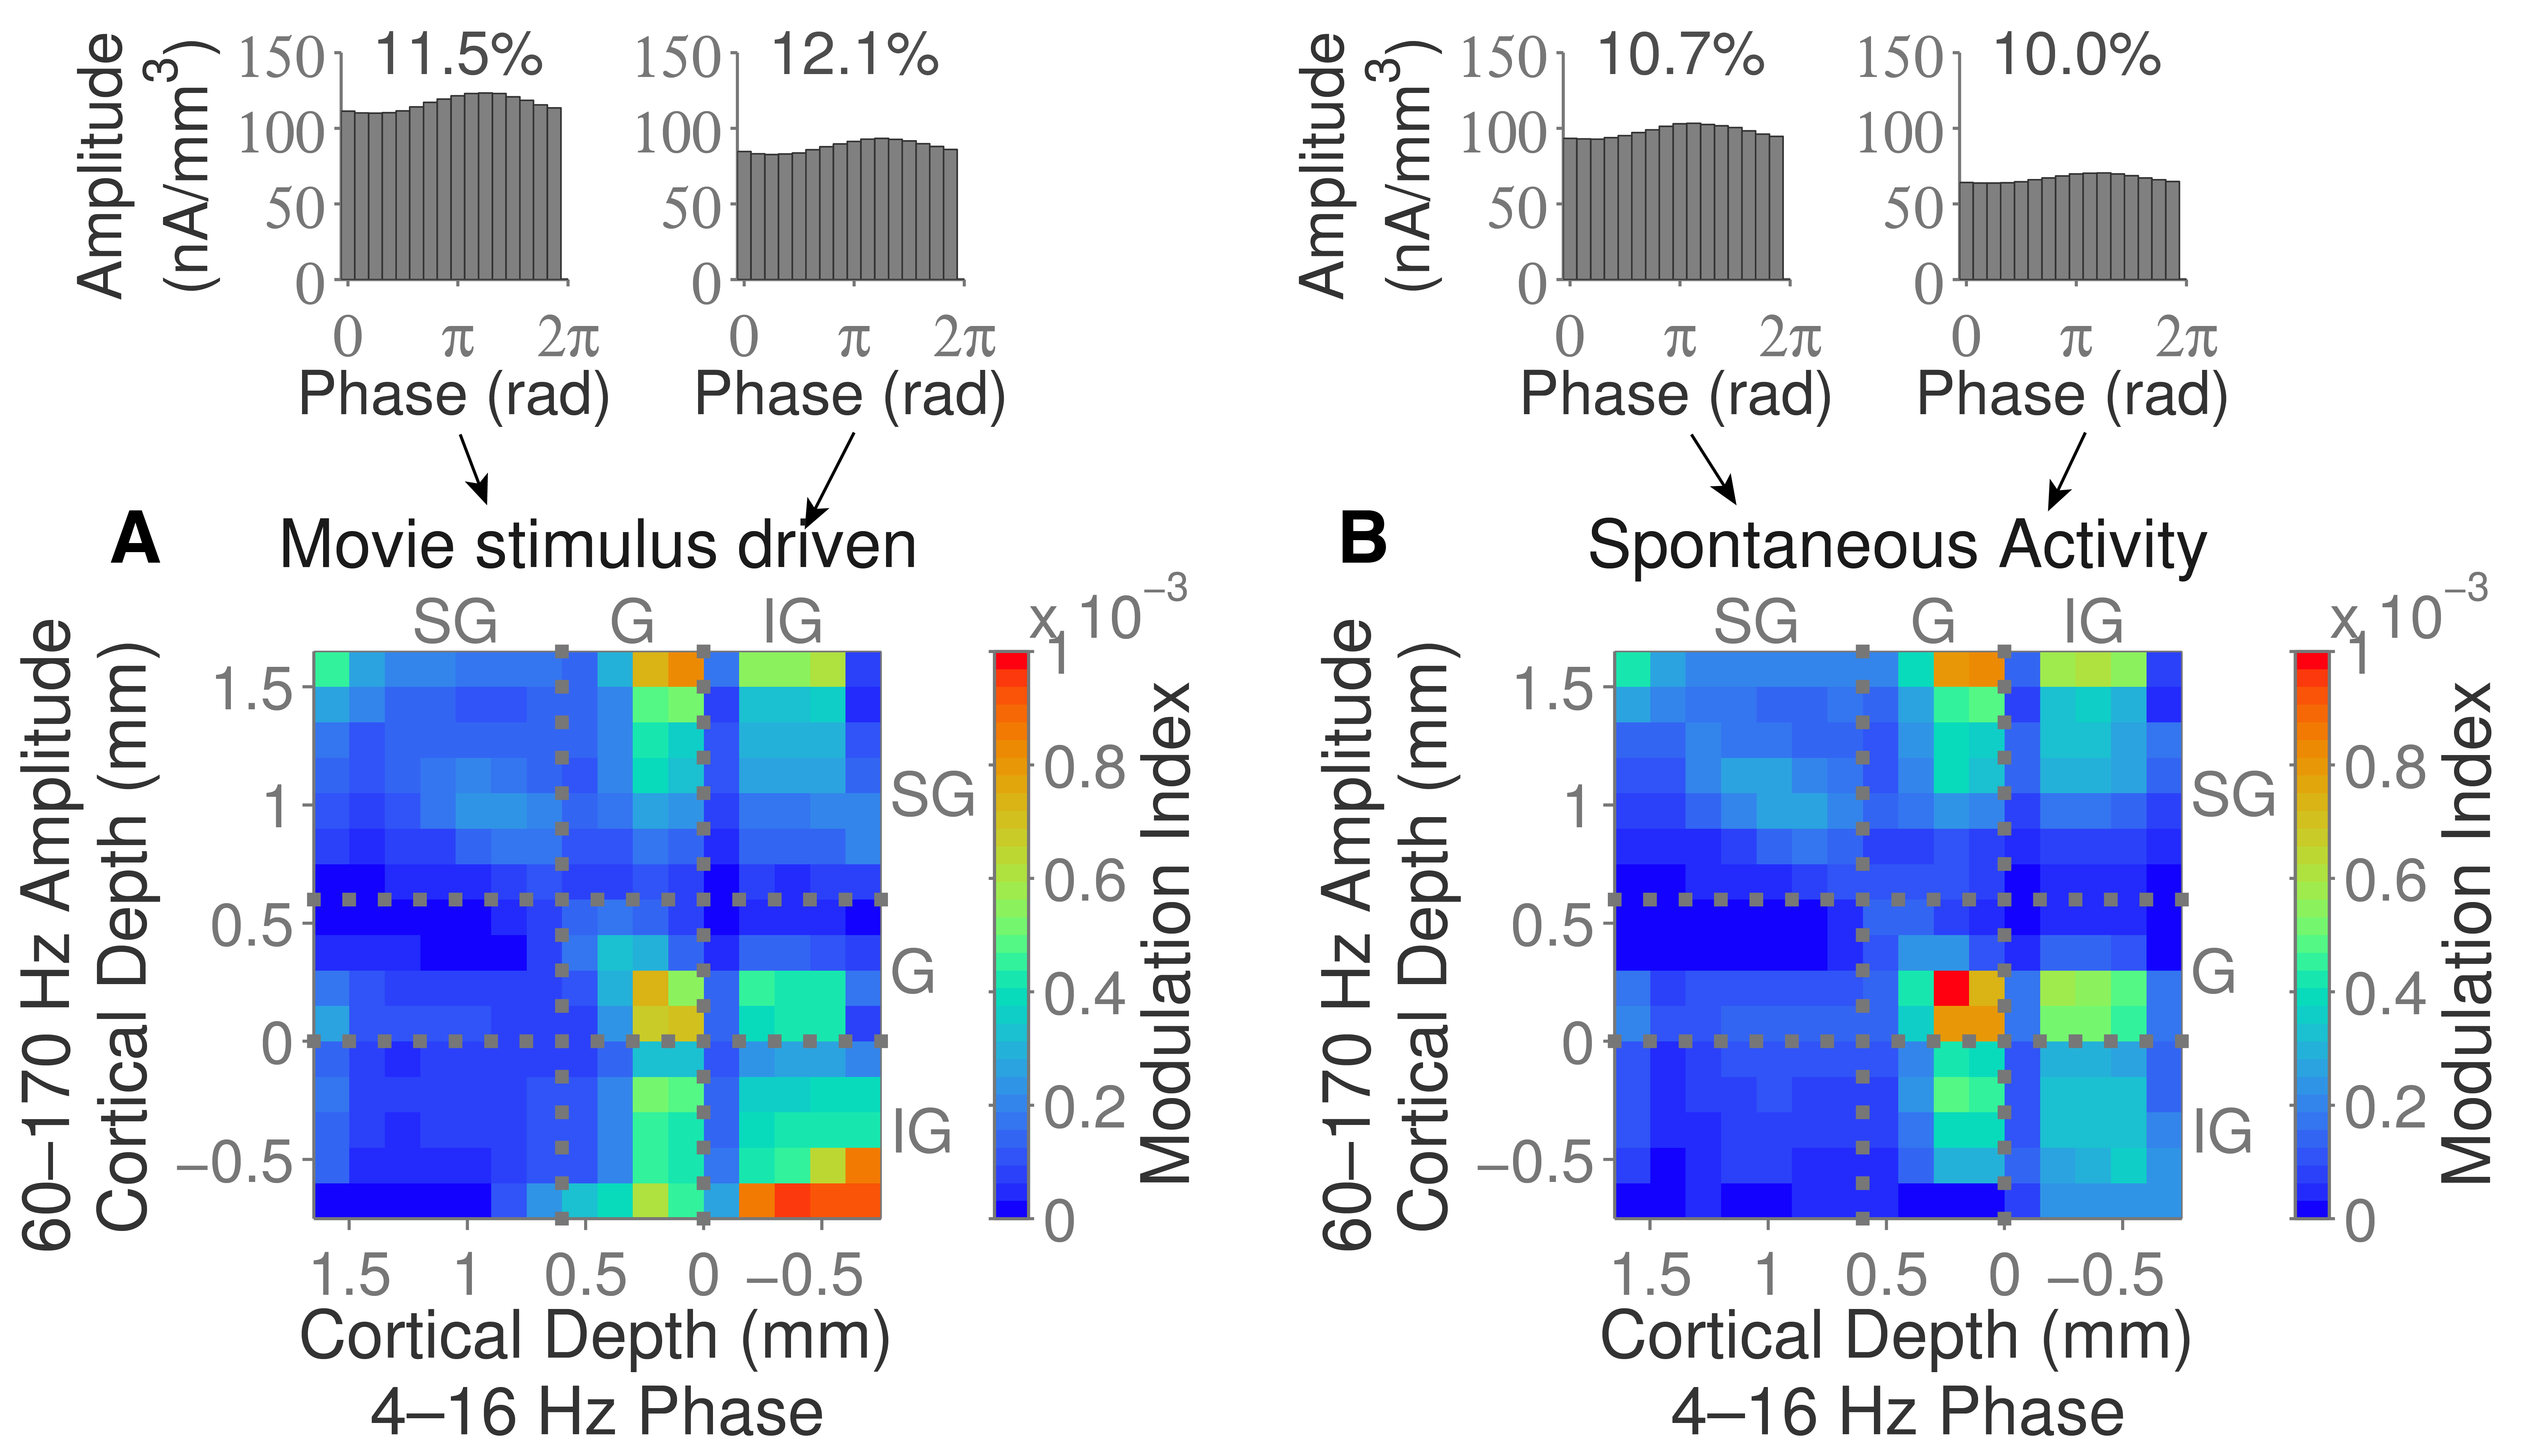
\includegraphics[width=\columnwidth]{paperfigs/fig8}
%
\caption{%
\textit{Cross-frequency phase-amplitude coupling}
Phase-amplitude modulation index between low frequency (\SIrange{4}{16}{Hz}) phase and high frequency (\SIrange{60}{170}{Hz}) amplitude (A: movie driven activity; B: spontaneous activity).
Mean of \num{5} sessions.
C and D: Amplitude as a function of binned phase for an example session (\sesname{H05391}), for \ac{IG}$\rightarrow$\ac{IG} coupling (left) and \ac{IG}$\rightarrow$\ac{SG} coupling (right).}%
\label{fig:lam_8}
%
\end{figure}


% =============================================================================
\section{Discussion}
% =============================================================================

In summary, we find while \ac{LFP} power is smooth and its depth profile is close to flat (Figures \ref{fig:lam_power_lfp} and \ref{fig:lam_power_csd}) the information that the \ac{LFP} encodes reveals much more structure.
We found there are two cortical regions at which oscillations in these frequency ranges are much more informative.
Namely \SIrange{4}{16}{Hz} at upper granular and mid-infragranular, and \SIrange{60}{170}{Hz} at upper supragranular and mid{}-infragranular regions.Previous work \citep{Belitski2008} has shown that in the macaque primary visual cortex information is coded in two frequency bands (\SI{<40}{Hz} and \SI{>40}{Hz}) containing independent information about natural visual scenes.
Our analysis extended across the cortical depth, and we found there are two cortical regions at which oscillations in these frequency ranges are much more informative (\SIrange{4}{16}{Hz} at upper-\ac{G} and mid-\ac{IG}; \SIrange{60}{170}{Hz} at upper-\ac{SG} and mid-\ac{IG} regions).

We also examined whether changes in luminance at different spatial frequencies induced differential changes in the cortex as a function of neural frequency and depth.
Namely, high spatial frequencies are encoded in oscillations faster than \SI{40}{Hz} and low spatial frequencies are encoded in oscillations slower than \SI{40}{Hz}.
We found that frequencies below and above \SI{40}{Hz} contain information about different spatial frequencies.

There are multiple, not mutually exclusive, possible interpretations of these findings.
Firstly, it is conceivable that the coding of different aspects of the stimulus into different frequency bands is a computational strategy of the cortex.
Our results suggest there is multiplexing in the cortex, with low frequency and high frequency oscillations of the same population activity simultaneously encoding low and high spatial frequency components of the stimulus respectively.
The idea of different frequency bands conveying different spatial frequency components of the stimulus has been proposed before from the results of an \ac{EEG} study \citep{Smith2006}.

One would expect that if certain oscillation frequencies in the visual cortex contain information about specific aspects of the stimulus, this is likely to be because the brain has encoded this information into oscillations in the activity of the local population.
This would only make sense if the information is utilized by the brain in order to interpret its stimuli.
Consequently, our results indicate there is multiplexing in the cortex, with low frequency and high frequency oscillations of the same population activity simultaneously encoding low and high spatial frequency components of the stimulus respectively.
Intuitively, information contained in the two frequency bands can be combined by downstream visual cortical regions to regain the original stimulus as necessary.
The idea of different frequency bands conveying different spatial frequency components of the stimulus has been proposed before from the results of an \ac{EEG} study \citep{Smith2006}.

Additionally, we can speculate about why separating the visual scene into low frequency (coarse) and high frequency (fine) components in \ac{V1} is useful.
One possibility is that low frequency oscillations are output from \ac{V1} along the dorsal visual stream, whereas high frequency oscillations travel propagate through the ventral stream [IS THERE EVIDENCE FOR THIS?].
Another possibility is that broad, coarse changes in the stimulus are useful for making rapid responses in the motor cortex to sudden changes, such as approaching threats.

Separation into low and high frequency domains with different properties seems to be a common property of the cortex.
In motor cortex, activity at \SI{<13}{Hz} and \SI{>60}{Hz} relates to behaviour but there is a separating band \SI{\approx30}{Hz} which does not \citep{Rickert2005}.
In the hippocampus, there is a gating effect between \SI{30}{Hz} and \SI{40}{Hz}, with lower but not higher frequencies able to propagate to the cortex \citep{Moreno2015}.
[also some unpublished research by Julian Hoffman into independent oscillations in the barrel cortex].
This suggests this encoding scheme is common across the cortex.
Some studies have suggested that the coupling of oscillations between two cortical regions facilitates the transmission between them [CITE SOME EXPERIMENTAL \& COMPUTATIONAL WORKS].

A separation of visual stimuli into coarse and fine channels is known to occur before the stimuli arrive in the cortex.
The outputs from different types of \acp{RGC} travel to the cortex through different regions of \iac{LGN}.
The M-pathway arises from \acp{RGC} with large, achromatic receptive fields, and projects mainly onto layer 4C$\alpha$ in \ac{V1}.
The P-pathway originates with \acp{RGC} with smaller, chromatic \acp{RF} providing higher spatial resolution but lower temporal resolution; this pathway projects onto layer 4C$\beta$ \citep{Callaway1998}.
It is possible that the two frequency channels in \ac{V1} relate to the two pathways providing its inputs.
[Cite Nathaniel J Killian from AREADNE on information in low-frequencies of \ac{LGN}.
Nothing available to actually cite?]

Since \ac{L4} is generally regarded as the primary layer of \ac{V1} which receives afferent inputs from \iac{LGN}, some readers might wonder how information in the gamma band has ``arisen'' in \ac{SG} layers without passing through \ac{G}.
However, our results do not necessitate this.
Fine-resolution information about the visual stimulus can arrive from the \ac{LGN} into \ac{L4} of \ac{V1}, with the information encoded into which neurons the afferent connections target.
This information is not detectable from the population level activity.


As many readers will be aware, it has long been known that neurons in the primary visual cortex have a response curve tuned to a preferred spatial frequency.
Work demonstrating the spatial frequency preference of single neurons typically involves the presentation of moving sinusoidal grating with a particular spatial frequency.
[NOT SURE WHERE I WAS GOING WITH THIS{\dots}]

The higher frequency band contains information about higher spatial frequencies changes in the stimulus.
This corresponds to the detection of edges and texture, which are properties that single neurons in \ac{V1} are known to be selective for.


We observed that each frequency has a similar amount of power across the cortical depth, but oscillations at these frequency ranges contain much more information at particular cortical depths.
This is curious as it indicates that, for any given frequency band, oscillations are present in all cortical depths, but most of the oscillations exhibited are not stimulus encoding.
This seems wasteful.
[important point]

We observed qualitatively that information-carrying events in \ac{L4} were large, temporary deflections with a long duration (low frequency), whereas \acs{L5/6} contained sustained oscillations (see \autoref{fig:lam_1}A for examples).
The deflections in \ac{L4} were usually coincident with scene cuts or rapid changes in the stimulus.
This could be interpreted as an error signal, since sudden, large changes in the stimulus would result in any predictive model of the stimulus making large errors.
However, a more simple interpretation is these deflections correspond to changes in the afferent input to \ac{V1} from \ac{LGN}.
In support of this, we note that the spatial scale of the information in the low frequency band (\SI{0.25}{\cpd}) approximately corresponds to the size of receptive fields for regions of the \ac{V1} corresponding to the parafovea (\SI{2}{\degree}).

The sustained oscillations in \acs{L5/6} also contain information about coarse changes in the stimuli.
These cortical layers are known to have connections to the motor cortex, feedback to \iac{LGN} and receiving feedback from higher cortical regions.


Recent work has indicated that alpha and gamma bands are important for feedback and feedforward activity respectively \citep{VanKerkoerle2014}.
This study \citep{VanKerkoerle2014} found that gamma waves are initiated at \ac{L4} and propagate outwards to the top of \ac{SG} and bottom of \ac{IG}, with alpha waves propagating in the opposite direction.
Our study finds the most information in gamma bands at the very top (and very bottom) of the cortex, and the most information in alpha bands at the top of \ac{L4} (and \ac{L6}).
Reconciling these results together, we find that there is most information in the power of the alpha and gamma oscillations at the cortical depths where they terminate, and the least where they originate.
This suggests that the oscillations are generated at one cortical depth without much stimulus dependency, but as the oscillations propagate up and down the cortex they are either amplified or supressed in a stimulus dependent manner.

In agreement with previous work \citep{Spaak2012}, we found there was cross-frequency coupling between the stimulus-encoding power of gamma oscillations in \ac{L1} and the phase of alpha oscillations in lower \ac{L4}.
Anatomically, we believe this is related to the pyramidal cell bodies in \ac{L5A}, which have apical dendritic tufts in \ac{L1} \citep{Hill2013,Zhu2004}.
This cross-frequency coupling could be one mechanism through which the \ac{L1} gamma wave containing high levels of information about the stimulus is converted into an alpha oscillation for feedback into the hierarchically lower cortical region.
Neurons in \ac{L5} are known to be related to long-range cortical output \citep{Hill2013}.
